%% Journal of Forecasting submission in Wiley's USG.cls (NJD authoring class, v6.0).
%% Build: pdflatex -> bibtex -> pdflatex -> pdflatex
\documentclass[ASNA]{USG}

\usepackage{amsmath}
\usepackage{booktabs}
\usepackage{threeparttable}
\usepackage{array}
\usepackage{graphicx}
\usepackage{xurl}
\usepackage{lineno}
\graphicspath{{images/}{./images/}}
\setlength{\emergencystretch}{2em}

\newcommand{\pkg}[1]{\textsf{#1}}
\newcommand{\proglang}[1]{\textsf{#1}}
\newcommand{\code}[1]{\texttt{#1}}
\providecommand{\sectionref}[1]{Section~\ref{#1}}
\providecommand{\tableref}[1]{Table~\ref{#1}}
\providecommand{\figureref}[1]{Figure~\ref{#1}}

\articletype{Research Article}
\received{}\revised{}\accepted{}
\journal{Journal of Forecasting}
\copyyear{2026}\volume{00}\startpage{1}\articledoi{10.1002/for.0000}

%% Required patches to the Wiley demo template (see the wiley-statistics-in-medicine skill):
%% (a) no "OPEN ACCESS" badge on a subscription submission; (b) no demo journal masthead.
\makeatletter
\def\@@articletype{%
  \rule[-4\@p@t]{4\@p@t}{15\@p@t}%
  \hskip -0\@p@t%
  {\arttypefont\bf\uppercase{\letterspace to 1.15\naturalwidth{\@articletype}}}%
}%
\makeatother
\usepackage{etoolbox}
\makeatletter
\patchcmd{\@maketitle}{
\includegraphics[width=56mm]{allergy.eps}}{}{}{}
\makeatother

\begin{document}

\title{Foundation or Formula? A Simulation-Based Comparison of Google's TimesFM-3 and Classical
Time-Series Models}

\author[1]{Ebrahim Khaled Ebrahim}[https://orcid.org/0009-0006-7839-8778]
\author[2]{Somaia Mohamed Ali}[https://orcid.org/0009-0002-0940-8451]
\author[3]{Ahmed El-Kotory}[https://orcid.org/0009-0000-1485-0768]
\authormark{EBRAHIM \textsc{et al.}}
\titlemark{TimesFM-3 versus classical models}

\address[1]{\orgdiv{Department of Applied Statistics, Faculty of Business},
\orgname{Alexandria University}, \orgaddress{\city{Alexandria}, \country{Egypt}}}
\address[2]{\orgdiv{Department of Statistics}, \orgname{Alexandria University},
\orgaddress{\city{Alexandria}, \country{Egypt}}}
\address[3]{\orgname{Alexandria University}, \orgaddress{\city{Alexandria}, \country{Egypt}}}

\corres{Ebrahim Khaled Ebrahim, Department of Applied Statistics, Faculty of Business,
Alexandria University, Alexandria, Egypt. \email{ebrahimkhaled@alexu.edu.eg}}

\keywords{Exponential smoothing | Forecast evaluation | Intermittent demand | Simulation study |
Time-series foundation models | Zero-shot forecasting}

\abstract[Abstract]{Time-series foundation models such as Google's TimesFM-3 forecast series they were never
trained on. Whether they should replace classical methods such as ARIMA and exponential smoothing is
difficult to settle on public benchmarks, because few benchmark datasets are absent from every
model's pre-training corpus. This exploratory study describes, under controlled conditions, how
TimesFM-3 behaves relative to classical methods and in which regimes it may be preferred. The
evaluation data are generated from nine known processes, so the model cannot have seen the series.
Across 7\,200 series and a pre-registered protocol with a 12-step horizon, neither family dominates.
TimesFM-3 is never more than 1.31 times worse than the best method in a cell, whereas every classical
method is at least 2.2 times worse somewhere; the largest classical failures occur with only two seasonal
cycles, where the automatic methods fall back to non-seasonal models, and without those cells automatic
ARIMA's worst case is 1.62. With four or more cycles automatic ARIMA is 21--24\% more accurate than
TimesFM-3 on seasonal ARIMA data. Among five foundation models, this
robustness is specific to TimesFM-3, and it is specific to short horizons: at 48 steps, TimesFM-3 and the
other foundation models forecast a decline on a saturating process whose level stays flat, and automatic
ARIMA has the smaller worst case elsewhere. On intermittent demand TimesFM-3 shows no advantage over
simple benchmarks built from the history. In post-hoc checks, randomised parameters, heavy-tailed noise and
outliers leave these patterns qualitatively unchanged, and on the official test period of 1\,000 M4
monthly series TimesFM-3 is level with the fifth- to seventh-ranked M4 entries, behind the four best, and
among ten methods whose ranks cannot be separated. Because TimesFM-3 is a black box, the study characterises
its behaviour, not the reasons for it; the findings are conditional on the processes and horizons examined,
and the model's weights are licensed for non-commercial use only.}

\maketitle
\setcounter{secnumdepth}{3}

\linenumbers


\section{Introduction}
\label{sec:intro}

Time-series foundation models are large neural networks, pre-trained on many series and then applied
to new series without task-specific training. On 31 August 2026 Google Research released TimesFM-3, a
330-million-parameter decoder-only transformer and the first member of its family designed for
multivariate forecasting, which its developers report as the top-ranked pre-trained model on three
public benchmarks \citep{timesfm3blog}, a claim open to the leakage concerns discussed next. For applied forecasting the relevant question is whether such a
model should be used, in preference to a classical method such as ARIMA, for the series at hand; the two
families also differ in cost, interpretability, the basis of their prediction intervals and the terms
under which they may be used (\sectionref{sec:operational}).

Published benchmarks are poorly suited to answering that question. Of 401 datasets used to evaluate
22 time-series foundation models, only about 6\% had never appeared in any model's pre-training
corpus, and even a 0.1\% overlap can move the mean absolute percentage error by 8 to 29 percentage
points \citep{meyer2025leakage}. Foundation-model evaluations have also been criticised for comparing
against under-tuned classical baselines rather than the combinations that win forecasting competitions
\citep{makridakis2020m4}. This study therefore generates its own evaluation data. Under a known
data-generating process (DGP) the foundation model cannot have seen the series, because they did not
exist before the experiment, and the model families searched by AutoARIMA and AutoETS contain the true
process of the linear and exponential-smoothing DGPs. What the design excludes is contamination at the
level of the realisation; what it cannot exclude is familiarity at the level of the family, because
TimesFM-3 is pre-trained partly on synthetic series \citep{timesfm3blog}. Such familiarity cannot be
measured here, and its direction cannot be assumed: synthetic corpora contain autoregressive and seasonal
structure, resembling D1--D5, but also level shifts, piecewise trends and sparse spikes, resembling
D6--D8. No conclusion of this paper relies on its direction.

The aim of the study is exploratory: to describe, under controlled conditions, how the accuracy of
TimesFM-3 relative to classical methods varies across regimes, and to derive diagnostic baselines for
when it may be preferred and when it should not. It proposes no new estimator, test or theory. The
design can establish what TimesFM-3 does but not why: the 330 million parameters have no individual
interpretation and the pre-training corpus cannot be inspected, so explanations of its behaviour offered
here are interpretations consistent with the measurements, not findings. The measurements concern one
model, one checkpoint and univariate zero-shot use, and they do not support general statements about
foundation models as a class.

TimesFM-3 is compared with seasonal naive, Theta, AutoETS, AutoARIMA and an equal-weight combination of
the last three on 7\,200 series from nine DGPs, four lengths from 24 to 200 observations and three
horizons, under a protocol written and frozen before any forecast was produced; every departure from it
is recorded. This pre-registered comparison is confirmatory in design; everything after it is post hoc
and exploratory, and is labelled as such. The evaluation is then extended with stronger benchmarks and two further foundation models,
tested for representativeness and robustness, and repeated on 1\,000 M4 monthly series.
\sectionref{sec:timesfm} describes TimesFM-3, \sectionref{sec:design} the design and
\sectionref{sec:results} the pre-registered results. \sectionref{sec:extended} extends the evaluation,
\sectionref{sec:robustness} examines representativeness and robustness, and \sectionref{sec:realdata}
turns to M4. \sectionref{sec:operational} covers operational considerations,
\sectionref{sec:discussion} discusses the evidence, and \sectionref{sec:conclusion} concludes;
reproducibility details are in \sectionref{sec:repro}.

\subsection{Related work}
\label{sec:related}

TimesFM \citep{das2024timesfm}, Chronos \citep{ansari2024chronos}, Moirai \citep{woo2024moirai},
TimeGPT \citep{garza2023timegpt} and Lag-Llama \citep{rasul2023lagllama} established that a single
pre-trained network can forecast unseen series zero-shot, and GIFT-Eval \citep{aksu2024gifteval} and
fev-bench \citep{shchur2025fevbench} supplied common benchmarks that include AutoARIMA, AutoETS and
seasonal naive among their baselines. The critical literature has grown alongside: \citet{meyer2025leakage}
on contamination, and \citet{adler2026calibrated}, who found on six public datasets that the calibration
error of five foundation models grows with forecast length. The present study differs from the latter in
using generated rather than public data, in testing accuracy differences with multiplicity control
rather than only summarising calibration, and in evaluating TimesFM-3. Applied comparisons on real data
are appearing in several fields---\citet{chu2026influenza} compare six foundation models with SARIMA on
influenza surveillance data---but they cannot say why a model works, because the generating mechanism is
unknown.

The design follows a pattern established in this journal, a controlled simulation over several DGPs
followed by an empirical application \citep{berger2025deep, chu2026intervals, lisi2025multiple}, and it
checks the realism of the simulated series in a feature space, as in \citet{kang2017instance} and
\citet{talagala2023metalearning}. AutoARIMA and AutoETS follow the Hyndman--Khandakar procedures
\citep{hyndman2008forecast, hyndman2002statespace}, Theta \citep{assimakopoulos2000theta} won M3 \citep{makridakis2000m3}, and the
combination is included because combinations are the standard against which competition entries are
judged \citep{makridakis2000m3, makridakis2020m4}. Evaluation follows the scale-free conventions of
\citet{hyndman2006mase} and the M5 competition \citep{makridakis2022m5, makridakis2022m5unc} and avoids
the pitfalls catalogued by \citet{hewamalage2023evaluation}.

\section{The TimesFM-3 model}
\label{sec:timesfm}

This section describes the architecture and pre-training data of TimesFM-3
(\sectionref{sec:tfm-architecture}) and the checkpoint and configuration used
(\sectionref{sec:tfm-config}).

\subsection{Architecture and pre-training data}
\label{sec:tfm-architecture}

TimesFM-3 is the third generation of the decoder-only TimesFM family \citep{das2024timesfm,
timesfm3blog}. Each input series is normalised by an iterative reversible instance normalisation, with
linear detrending of strongly trending inputs, and divided into non-overlapping patches of 32 time points,
each embedded as a token; 20 transformer layers with model dimension 1280 and 16 attention heads give
about 330 million parameters (the checkpoint loaded here has 330\,710\,976). Layers of causal attention
along time alternate with layers of attention across variates, so target series and covariates can be
processed jointly, and a contiguous patch masking scheme produces the whole horizon in one forward pass,
in output patches of 64 points. For each step the model returns nine quantiles, the 10th to the 90th
percentile, and its point forecast is the median \citep{timesfm3blog, timesfm3card, timesfm3repo}. These
details come from the developers' blog post and model card and from the configuration file of the
checkpoint (accessed 23 September 2026); none has yet been described in a peer-reviewed publication. The
pre-training corpus of more than one trillion time points combines the GIFT-Eval pre-training collection,
Wikipedia page views to November 2023, Google Trends queries to the end of 2022, and synthetic and
augmented series \citep{timesfm3card}.

\subsection{Checkpoint and configuration}
\label{sec:tfm-config}

The weights (\code{google/\allowbreak timesfm-3.0-pytorch} on the Hugging Face Hub, revision
\code{43046b8}) are loaded with version 3.0.1 of the \pkg{timesfm} \proglang{Python} package, which provides
both the \code{timesfm} and \code{timesfm3} modules \citep{timesfm3repo, timesfm3card}, and are licensed for
non-commercial use only (\sectionref{sec:operational}). The model is used zero-shot: it receives only the
raw context, with no fine-tuning, covariates or seasonal period, through \code{predict\_batch} with its
default settings (no symmetric averaging, no positivity constraint, 32-bit arithmetic). Its point forecast is
the model's own median output; the nine deciles are then sorted, which matters only where they cross
(\sectionref{sec:tfm-check}). A context shorter than the model's working length is left-padded with zeros
and masked, so at $n = 24$ the model sees one partly filled patch; the package's maximum context of
15\,360 points truncates no series in this study, and a series forecast alone or inside a batch of other
lengths gives quantiles that agree to within $2 \times 10^{-5}$. Because no quantile outside the 10th and
90th percentiles is available, the widest interval that can be formed is the nominal 80\% interval. The
weights, code and revision are public, so every forecast can be regenerated (\sectionref{sec:repro}); the
developers' own evaluator settings are examined in \sectionref{sec:tfm-check}.

\section{Design of the simulation study}
\label{sec:design}

This section describes the data-generating processes (\sectionref{sec:dgps}), the forecasting
methods compared (\sectionref{sec:methods}), and the evaluation measures and inferential
procedures (\sectionref{sec:evaluation}). \tableref{tab:ademp} summarises the design in the
aims--data--estimands--methods--performance form recommended for simulation studies by
\citet{morris2019simulation}.

\begin{table}[!htbp]
\centering
\begin{threeparttable}
\caption{Structure of the simulation study.}
\label{tab:ademp}
\small
\begin{tabular}{>{\raggedright\arraybackslash}p{2.6cm}>{\raggedright\arraybackslash}p{11.4cm}}
\toprule
Element & Specification \\
\midrule
Aims & Describe how the accuracy of zero-shot TimesFM-3 relative to classical methods varies across
  known data-generating regimes; exploratory. \\[2pt]
Data-generating mechanisms & Main design: nine processes (\tableref{tab:dgps}) with fixed
  parameters, $n \in \{24, 48, 96, 200\}$, $H = 12$, 200 replications per cell. Robustness design
  (\sectionref{sec:departures}): parameters drawn per series from wide ranges (Table~S8), four versions
  (Gaussian, heavy-tailed, outliers, tested seasonality), 200 replications per cell. \\[2pt]
Estimands & For each method and cell: the expected MASE over $h = 1, \dots, 12$ (and RMSSE, scaled
  pinball loss, 80\% coverage); for each pair of methods and cell: the pseudo-median of the paired
  MASE difference. Summaries across cells (worst ratio, win counts) were defined post hoc. \\[2pt]
Methods & Seasonal naive, Theta, AutoETS, AutoARIMA, their combination and TimesFM-3 (pre-registered);
  DOTM, the M4 Comb benchmark, a second combination, TimesFM-2.5, Chronos-Bolt and the Croston family
  (post hoc). \\[2pt]
Performance measures & Mean MASE with its Monte Carlo standard error; ratio to the best method in
  a cell, with bootstrap intervals for summaries across cells; paired Wilcoxon tests with
  Hodges--Lehmann estimates and Benjamini--Hochberg control; coverage and width of 60\% and 80\%
  intervals. With 200 replications the Monte Carlo standard error of a paired MASE difference is about
  2\% of the mean (\sectionref{sec:effects}). \\
\bottomrule
\end{tabular}
\begin{tablenotes}[flushleft]\footnotesize
\item \textit{Note:} The mean MASE (descriptive) and the pseudo-median difference (inferential)
are different estimands and can disagree when the error distribution is skewed, as on the
intermittent process D8 (\sectionref{sec:effects}); both are reported.
\end{tablenotes}
\end{threeparttable}
\end{table}

\subsection{Data-generating processes}
\label{sec:dgps}

Nine processes were chosen to span the range from ``a classical model is exactly right'' to
``no classical model is right''. \tableref{tab:dgps} lists them. Each series is generated at
length $n + H$ with $H = 12$; the first $n$ observations form the context supplied to every
method, and the final 12 are held out as the truth. One realisation of each process is shown
in \figureref{fig:series}.

\begin{table}[!htbp]
\centering
\begin{threeparttable}
\caption{The nine data-generating processes and their parameters.}
\label{tab:dgps}
\small\setlength{\tabcolsep}{4pt}
\begin{tabular}{llll}
\toprule
ID & Data-generating process & Parameters & Correctly specified by \\
\midrule
D1 & AR(1)                        & $\phi = 0.7$                                & ARIMA \\
D2 & ARMA(1,1)                    & $\phi = 0.6$, $\theta = 0.4$                & ARIMA \\
D3 & ARIMA(1,1,1) with drift      & $\phi = 0.5$, $\theta = 0.3$, drift $0.3$   & ARIMA \\
D4 & SARIMA(1,0,0)(1,1,0)$_{12}$  & $\phi = 0.6$, $\Phi = 0.5$                  & ARIMA \\
D5 & ETS(A,A,A)                   & $\alpha = 0.3$, $\beta = 0.01$, $\gamma = 0.2$ & ETS \\
D6 & Local level with a break     & break at $0.7n$, jump $10\sigma$            & neither \\
D7 & Logistic growth              & $K = 180$, $r = 0.08$, floor $20$           & neither \\
D8 & Intermittent demand          & $p = 0.3$, size $1 + \mathrm{Pois}(4)$      & neither \\
D9 & AR(1) with GARCH(1,1) errors & $\phi = 0.6$, $a = 0.1$, $b = 0.85$         & ARIMA in mean \\
\bottomrule
\end{tabular}
\begin{tablenotes}[flushleft]\footnotesize
\item \textit{Note:} The last column states which classical family is correctly specified by
construction; for D6--D8 none is, and for D9 the conditional mean is correctly specified while
the conditional variance is not. Innovations are Gaussian with standard deviation $\sigma = 2$ ($\sigma = 3$
in D7; D8 has none). D1, D2 and D9 fluctuate about a mean of 100 after a burn-in of 300 steps (D9:
$\omega = 0.1$); D3 starts at 100 after its differences are burnt in; D4 starts from the cycle
$100 + 10\sin(2\pi k/12)$ plus noise, its seasonal differences burnt in; D5 starts from level 100, trend
0.2 and seasonal states $10\sin(2\pi k/12)$; in D6 the level is a random walk from 100 with innovation
standard deviation 0.5 and $\sigma$ is that of the observation noise; D7 has lower asymptote 20; in D8 a
demand occurs with probability $p$.
\end{tablenotes}
\end{threeparttable}
\end{table}

\begin{figure}[!htbp]
\centering
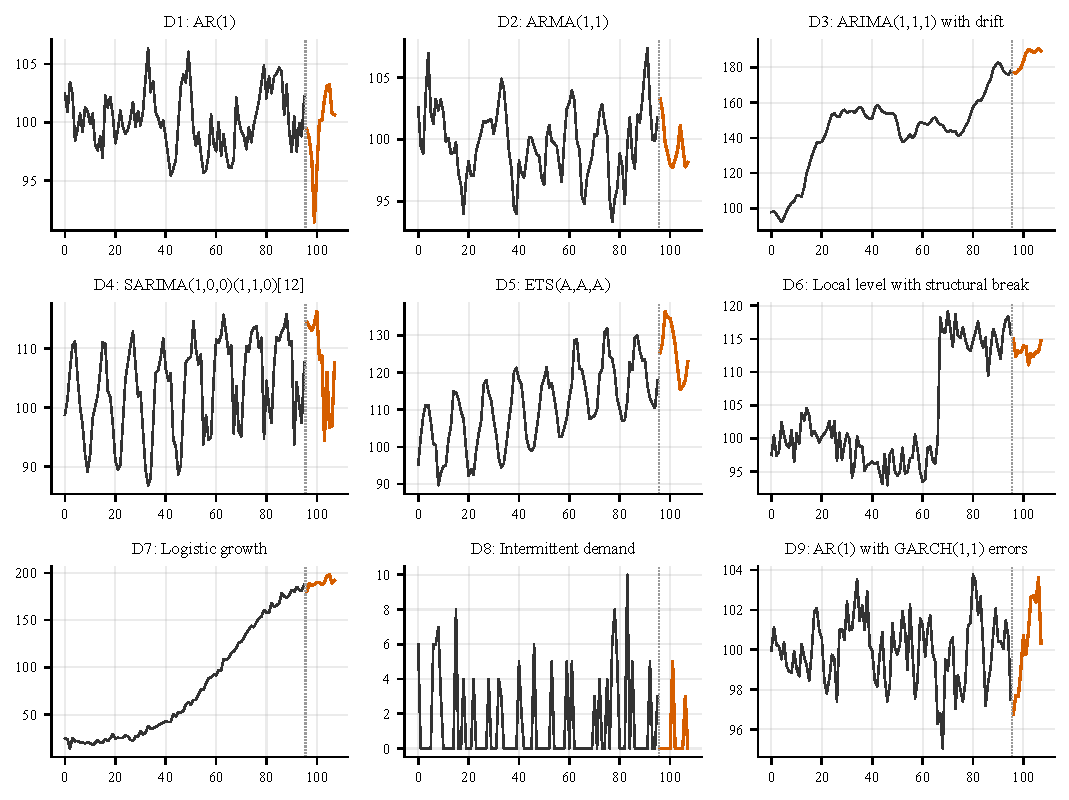
\includegraphics[width=\textwidth]{../figures/fig1_example_series.pdf}
\caption{One realisation of each data-generating process at $n = 96$. The context supplied to
every method is in grey and the held-out horizon in colour, separated by the dotted line.}
\label{fig:series}
\end{figure}

The parameter values in \tableref{tab:dgps} were fixed in the pre-registered protocol, each chosen so
that its process represents its regime unambiguously. The linear processes D1--D4 and the conditional
mean of D9 use coefficients no larger than 0.7 in absolute value, well inside the stationarity and
invertibility regions \citep{brockwell2016introduction}. The smoothing parameters of D5 lie inside the
usual region $0 < \beta < \alpha < 1$, $0 < \gamma < 1 - \alpha$ \citep{hyndman2008ets}, with a small trend
parameter so that the level stays positive. The break in D6 equals ten noise standard deviations, so the
comparison concerns adaptation to the break rather than its detection \citep{pesaran2007breaks}; D7
follows the logistic curve, the standard model of saturating growth \citep{meade2006diffusion}. In D8 the
mean interval between demands is $1/0.3 \approx 3.3$ periods and the squared coefficient of variation of
the sizes is $4/25 = 0.16$, so against the cut-offs of \citet{syntetos2005categorization} the process is
intermittent rather than lumpy, the regime for which Croston's method was developed \citep{croston1972}.
The GARCH(1,1) errors of D9 \citep{bollerslev1986garch} have persistence $a + b = 0.95$, strongly
persistent but covariance-stationary \citep{engle1986persistence}, a standard benchmark specification in
volatility forecasting \citep{hansen2005garch}. Every series has a level of about 100, or a positive lower
asymptote in D7, so percentage errors are defined except where zeros are intrinsic (D8); the trend
parameter of D5 and the asymptote of D7 were adjusted for this reason before any forecast was produced.
Because the conclusions could depend on these values, \sectionref{sec:robustness} repeats the comparison
with parameters drawn at random.

Three design choices need a word. The break in D6 is placed inside the context, at $0.7n$: a break in the
held-out window is unforecastable by any method, whereas one in the context asks whether a method
forecasts from the new level or reverts to the old one. The inflection of D7 sits at $0.6(n+H)$, so the
held-out window lies in the saturating arm, where a method that fits a linear drift overshoots. And the
shortest length, $n = 24$, leaves a seasonal model only two cycles from which to estimate its seasonal
structure, which separates whether a model is correctly \emph{specified} from whether it is
\emph{estimable}. Two hundred replications per (DGP, length) cell give $9 \times 4 \times 200 = 7\,200$
series, each seeded from its own identifiers.

\subsection{Forecasting methods}
\label{sec:methods}

No method is tuned by hand; each classical model uses its own automatic selection, the comparison a
practitioner faces. The classical models are fitted with \pkg{StatsForecast} \citep{statsforecast} at its
default settings, stated because the results depend on them. AutoARIMA searches stepwise over $p, q \le 5$
and $P, Q \le 2$ with $p + q + P + Q \le 5$, chooses $d \le 2$ and $D \le 1$ by unit-root tests, allows a
mean or drift and selects by AICc; AutoETS searches the full error--trend--season space (\code{ZZZ}) with
damped and undamped trends by AICc; Theta is the standard theta method with classical multiplicative
seasonal adjustment \citep{hyndman2021fpp}. The equal-weight combination of Theta, AutoETS and AutoARIMA
is included because the classical state of the art is a combination \citep{makridakis2020m4,
petropoulos2022theory}. Its point forecast is the mean of the members' forecasts and its quantiles the
decile-by-decile mean of theirs (vincentization), which gives a narrower distribution than a mixture when
the members disagree.

Every classical method receives the true seasonal period ($m = 12$ on D4 and D5, $m = 1$ elsewhere),
whereas TimesFM-3 receives only the raw context. This reflects ordinary practice---an analyst usually knows
that data are monthly---but it favours the classical methods on D4 and D5 once enough cycles are
observed; with two cycles they rarely use it (\sectionref{sec:estimability}).
\sectionref{sec:robustness} examines the alternative of testing for seasonality.

\subsection{Evaluation measures and statistical inference}
\label{sec:evaluation}

Point accuracy is measured mainly by the mean absolute scaled error \citep[MASE;][]{hyndman2006mase}.
With context $y_1, \dots, y_T$ ($T = n$), horizon $H$ and point forecasts $\hat{y}_{T+h}$,
\begin{equation}
\label{eq:mase}
\text{MASE} = \frac{\frac{1}{H}\sum_{h=1}^H |y_{T+h} - \hat{y}_{T+h}|}{\frac{1}{T-m}\sum_{t=m+1}^T |y_t - y_{t-m}|},
\end{equation}
so the scale is the in-sample seasonal-naive error for the seasonal processes and the naive error for the
others ($m = 12$ throughout for the M4 tier, as in M4). The root mean squared scaled error (RMSSE) replaces
absolute by squared errors in both numerator and denominator and takes the square root, and sMAPE is the
symmetric percentage error of the M4 competition. MAPE is undefined when an actual value is zero, which
happens only on D8 (in 9.96\% of all evaluations over the three horizon slices), and is reported only
in the Supporting Information (Section~S1) \citep{hyndman2006mase, kolassa2016count}.
Probabilistic accuracy is measured by a strictly proper scoring rule \citep{gneiting2007scoring}, the
pinball loss over the nine deciles $\tau \in \{0.1, \dots, 0.9\}$ scaled by the same denominator,
\begin{equation}
\label{eq:spl}
\text{SPL} = \frac{\frac{1}{9H} \sum_{\tau} \sum_{h=1}^H \max\{\tau(y_{T+h} - \hat{q}^{(\tau)}_{T+h}),\, (1-\tau)(\hat{q}^{(\tau)}_{T+h} - y_{T+h})\}}{\frac{1}{T-m}\sum_{t=m+1}^T |y_t - y_{t-m}|},
\end{equation}
where $\hat{q}^{(\tau)}_{T+h}$ is the $\tau$-quantile forecast, together with the coverage and width of
the nominal 60\% and 80\% intervals \citep{gneiting2007calibration}. Wider intervals cannot be formed from
TimesFM-3's nine deciles, so $[q_{0.1}, q_{0.9}]$ is the widest interval compared; classical quantiles are
taken from intervals at levels 20, 40, 60 and 80, which map onto the same deciles.

Within each (DGP, length) cell and horizon slice ($h = 1$, $1$--$6$ and $1$--$12$), TimesFM-3 is compared with each classical method by a paired
Wilcoxon signed-rank test \citep{wilcoxon1945} on per-replication MASE differences, with the
Hodges--Lehmann estimate \citep{hodges1963} and the median MASE ratio as effect sizes, and the
Benjamini--Hochberg procedure at a false discovery rate of 0.05 within each opponent family of 108
tests (36 cells and three slices), as pre-registered \citep{benjamini1995fdr}; the results report the
$h = 1$--12 slice. The Diebold--Mariano test \citep{diebold1995comparing} is not used: the
replications are independent, so there is no serial dependence for it to model, and in the real-data tier
three rolling origins per series leave it without power even with small-sample corrections
\citep{harvey1997testing}. The pre-registered protocol had reserved it for that tier; the departure is
recorded.

\section{Simulation results}
\label{sec:results}

This section reports the pre-registered comparison: overall accuracy and the pairwise tests
(\sectionref{sec:overall}), effect sizes (\sectionref{sec:effects}), the role of estimability
(\sectionref{sec:estimability}), the seasonal and intermittent regimes (\sectionref{sec:regimes}), and
interval coverage and the combination rule (\sectionref{sec:coverage}). Statements about TimesFM-3
describe the behaviour of its forecasts; where an explanation is offered, it is an interpretation.
\figureref{fig:ratio} shows TimesFM-3 relative to the best classical method in each of the 36
(process, length) cells; the mean MASE of every method in every cell, over $h = 1, \dots, 12$ and 200
replications, is given in Table~S9 of the Supporting Information.


\begin{figure}[!htbp]
\centering
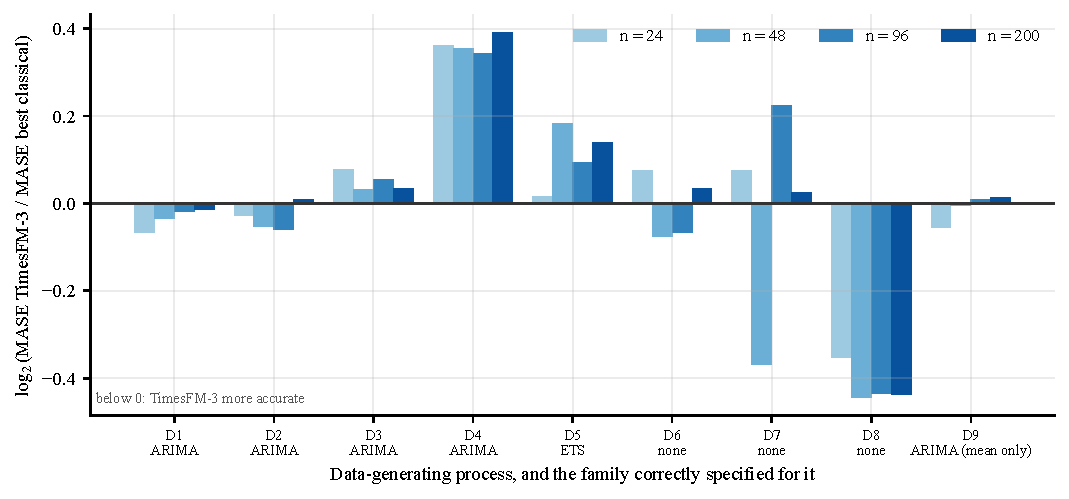
\includegraphics[width=\textwidth]{../figures/fig2_mase_ratio.pdf}
\caption{Accuracy of TimesFM-3 relative to the best classical method in each cell, on a
$\log_2$ scale. Bars below zero mark cells where TimesFM-3 is more accurate. The label under
each process names the family correctly specified for it by construction.}
\label{fig:ratio}
\end{figure}

\subsection{Overall accuracy and pairwise comparisons}
\label{sec:overall}

TimesFM-3 has the lowest mean MASE in 16 of the 36 (DGP, length) cells and the classical methods in 20:
AutoARIMA 10, seasonal naive 4, and two each for Theta, AutoETS and the combination. Against the best
classical method of each cell, 18 differences survive Benjamini--Hochberg correction, 7 favouring
TimesFM-3 and 11 the classical method; because that comparator is selected on the same replications,
these $p$-values are descriptive only. The inferential claims rest on the 180 comparisons with a fixed
opponent (\tableref{tab:opponents}): 132 are significant, 113 favouring TimesFM-3. These counts summarise
the tests; they weight every cell equally and depend on the mix of processes, and pooling the tests into a
single family changes them by at most two (Supporting Information, Section~S6). \textbf{AutoARIMA is the
only classical method that TimesFM-3 does not clearly beat}; against every other method, the combination
included, TimesFM-3 wins the large majority of significant comparisons.

\begin{table}[!htbp]
\centering
\begin{threeparttable}
\caption{Significant pairwise comparisons of TimesFM-3 with each classical method at
$h = 1,\dots,12$.}
\label{tab:opponents}
\small
\begin{tabular}{lccc}
\toprule
Opponent & Significant comparisons & TimesFM-3 wins & Opponent wins \\
\midrule
AutoARIMA          & 20 & 11 & 9 \\
Seasonal naive     & 26 & 22 & 4 \\
AutoETS            & 27 & 25 & 2 \\
Theta              & 29 & 28 & 1 \\
Combination        & 30 & 27 & 3 \\
\bottomrule
\end{tabular}
\begin{tablenotes}[flushleft]\footnotesize
\item \textit{Note:} Paired Wilcoxon signed-rank tests in the 36 (process, length) cells at
$h = 1, \dots, 12$, Benjamini--Hochberg corrected within each opponent family of 108 tests (three
horizon slices).
\end{tablenotes}
\end{threeparttable}
\end{table}

\begin{figure}[!htbp]
\centering
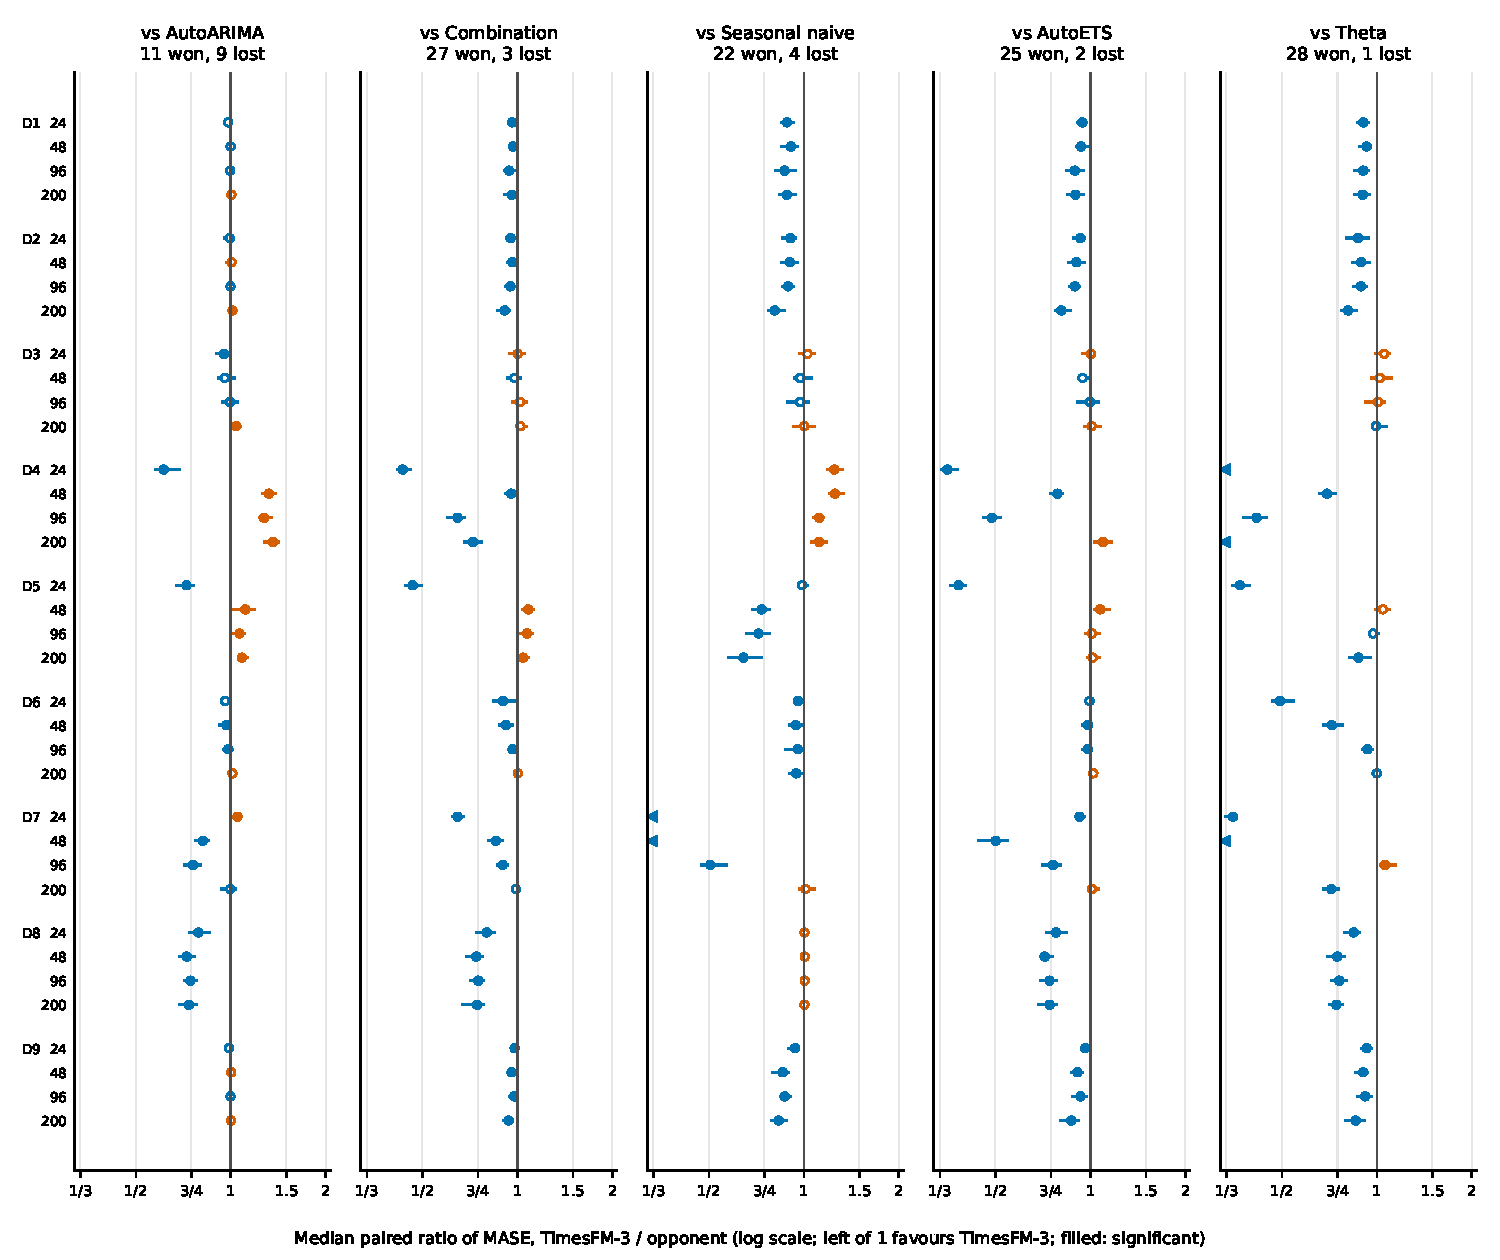
\includegraphics[width=\textwidth]{../figures/fig5_forest.pdf}
\caption{Pairwise comparisons of TimesFM-3 with each classical method, cell by cell: median of the paired
per-series ratios of MASE over $h = 1, \dots, 12$, with 95\% bootstrap intervals, on a logarithmic scale.
Filled markers are significant after Benjamini--Hochberg correction; points left of 1 favour TimesFM-3.
Arrowheads mark medians beyond the plotted range.}
\label{fig:forest}
\end{figure}


\figureref{fig:forest} shows the effect behind each count: against AutoARIMA most intervals straddle
1, and the cells where AutoARIMA is ahead are the seasonal processes from $n = 48$, whereas against the other
methods most intervals lie wholly on the side of TimesFM-3.

\subsection{Effect sizes and sensitivity to the choice of test}
\label{sec:effects}

The median Hodges--Lehmann shifts in MASE across the 36 cells are $-0.010$ against AutoARIMA, $-0.091$
against the combination, $-0.133$ against seasonal naive, $-0.183$ against AutoETS and $-0.227$ against
Theta (negative favours TimesFM-3), so against AutoARIMA the typical difference is about one hundredth of a
MASE unit. The Monte Carlo standard error of the paired difference between TimesFM-3 and AutoARIMA is 0.8\%
to 4.8\% of AutoARIMA's mean MASE (median 2.1\%), so differences smaller than about 6\% are unlikely to be
detected in a cell: the 11--9 split against AutoARIMA sits at the resolution of the design and does not show
that the two methods are equivalent. A paired $t$-test agrees with the Wilcoxon test in 163 of 180
comparisons (90.6\%). The largest block of disagreements is on the intermittent process D8 against seasonal
naive: the $t$-test finds TimesFM-3 better at every length ($p < 0.0001$), the signed-rank test finds no
difference ($p = 0.11$ to $0.92$). The mean difference is driven by a minority of series on which seasonal
naive fails badly, whereas on 64.5--72.0\% of series TimesFM-3 is marginally less accurate---the two tests
estimate different quantities of a heavily skewed error distribution (\tableref{tab:ademp}).

\subsection{Correct specification versus estimability}
\label{sec:estimability}

Pre-registered hypothesis H1 held that correctly specified classical models would win on their home
ground, most clearly at short lengths; \textbf{it is not supported in that form}. On D1 and D2 TimesFM-3 is
at least as accurate as the correctly specified AutoARIMA at every length except D2 at $n = 200$, the only
significant difference. Correct specification bought AutoARIMA nothing detectable on short and moderate
series. A post-hoc \emph{Oracle ARIMA}, which knows the true orders and estimates only the parameters by
Gaussian maximum likelihood, is consistent with order selection being the cost: on D1--D3 at $n = 24$
AutoARIMA pays a 9.9\% to 13.9\% penalty for selecting the orders, while the oracle beats TimesFM-3 in 15 of
the 16 ARIMA cells (for example 1.351 against 1.417 on D1 at $n = 24$). On D4 at $n = 24$ most oracle fits
did not converge (156 of 200, used as returned), so that cell is not interpreted.

The seasonal processes show the effect most clearly. With two complete cycles ($n = 24$), AutoETS scores
a mean MASE of \textbf{3.03 on D5, data an ETS process generated}, against 1.14 for seasonal naive and 1.15
for TimesFM-3: the correctly specified model has 2.7 times the error of the naive rule. The failure is not an
over-fitted seasonal model but the absence of one: given $m = 12$ and 24 observations, AutoETS chose a
seasonal form for 8.5\% of the D4 series and none of the D5 series, and AutoARIMA for none (Supporting
Information, Table~S11), whereas seasonal naive applies the known period without estimating anything. The
operative distinction is therefore whether a model is \emph{estimable} from the series at hand, not whether
it is correctly specified. \tableref{tab:robust} quantifies the resulting asymmetry with each method's mean
MASE as a multiple of the best in the same cell---a relative measure, because D3 is hard for every method
and would dominate absolute worst cases. \textbf{TimesFM-3 is never worse than $1.31\times$ the best method
of a cell}, and within 0.8\% of it in the median cell, whereas every classical method is at least $2.2\times$
worse somewhere: AutoARIMA $2.22\times$ and AutoETS $3.50\times$ (both on D4 at $n = 24$), Theta
$4.69\times$, seasonal naive $5.65\times$. Leaving out the two cells with two seasonal cycles, TimesFM-3's
worst ratio is unchanged and AutoARIMA's falls to 1.62 (on D7 at $n = 96$), AutoETS's to 2.72 and the
combination's to 2.08; the last two come from AutoETS on D4 at $n = 96$, a cell in which StatsForecast's
estimation fails (\sectionref{sec:regimes}), and with the value of R's \pkg{forecast} package there AutoETS's
worst ratio would be 2.13, on D7 at $n = 48$. The worst ratio is a descriptive summary defined after the protocol, and it depends on
the methods compared, notably on seasonal naive with the known period (\sectionref{sec:departures}).

% generated by code/K9_round2_revisions.py
\begin{table}[!htbp]
\centering
\begin{threeparttable}
\caption{Mean MASE relative to the best method in the same scenario, summarised over the 36 scenarios.}
\label{tab:robust}
\small\setlength{\tabcolsep}{4pt}
\begin{tabular}{lrrrlrl}
\toprule
 & & & \multicolumn{2}{c}{All 36 scenarios} & \multicolumn{2}{c}{Without the two-cycle scenarios} \\
\cmidrule(lr){4-5}\cmidrule(lr){6-7}
Method & Median & Mean & Worst & Scenario & Worst & Scenario \\
\midrule
Seasonal naive & 1.200 & 1.470 & 5.65 & D7 $n=48$ & 5.65 & D7 $n=48$ \\
Theta & 1.251 & 1.614 & 4.69 & D4 $n=200$ & 4.69 & D4 $n=200$ \\
AutoETS & 1.194 & 1.366 & 3.50 & D4 $n=24$ & 2.72 & D4 $n=96$ \\
AutoARIMA & 1.032 & 1.137 & 2.22 & D4 $n=24$ & 1.62 & D7 $n=96$ \\
Combination & 1.108 & 1.273 & 3.00 & D4 $n=24$ & 2.08 & D4 $n=96$ \\
\textbf{TimesFM-3} & \textbf{1.008} & \textbf{1.054} & \textbf{1.31} & D4 $n=200$ & \textbf{1.31} & D4 $n=200$ \\
\bottomrule
\end{tabular}
\begin{tablenotes}[flushleft]\footnotesize
\item \textit{Note:} Each entry divides a method's mean MASE by the lowest mean MASE in the same (process,
length) scenario, so a value of 1.00 means that the method was the best in that scenario; the mean is arithmetic.
The two-cycle scenarios are D4 and D5 at $n = 24$. Geometric means and 90th percentiles are in the Supporting
Information, Table~S9.
\end{tablenotes}
\end{threeparttable}
\end{table}


\subsection{Seasonal and intermittent regimes}
\label{sec:regimes}

\textbf{Strong seasonality with sufficient data (D4).} At $n = 48$, 96 and 200 AutoARIMA's mean MASE is
21.8\%, 21.1\% and 23.7\% below TimesFM-3's (adjusted $p < 0.0001$), and D5 shows the same more mildly (4\%
to 12\%). Once at least four cycles are observed, AutoARIMA recovers the seasonal structure and TimesFM-3
does not match it; seasonal naive, which estimates nothing, is also more accurate than TimesFM-3 on D4 at
every length (1.005 to 1.053 against 1.124 to 1.321). With two cycles the ranking among the others reverses:
TimesFM-3 beats AutoARIMA by 42\% (1.321 against 2.284). Theta deteriorates on D4 as the series
lengthens (Theta 1.94 at $n = 48$ and 4.16 at $n = 200$). D4 is seasonally integrated, so its seasonal
pattern drifts, whereas classical decomposition estimates one fixed pattern from the whole history; with
additive instead of multiplicative decomposition the failure is almost unchanged (in a check on 60
replications, Theta's mean MASE at $n = 200$ was 3.83 against 3.95), so it concerns the model form rather
than the adjustment.

Because the classical results could depend on the implementation, the D4 and D5 cells were refitted with
\code{auto.arima}, \code{ets} and \code{thetaf} of the \proglang{R} package \pkg{forecast}
\citep{hyndman2008forecast}, the reference implementation of the Hyndman--Khandakar procedures (post hoc;
Supporting Information, Table~S13). R reproduces every failure discussed here---AutoARIMA 2.87 and AutoETS
3.95 on D4 at $n = 24$, AutoETS 3.30 on D5 at $n = 24$, Theta 4.09 on D4 at $n = 200$---and, like
StatsForecast, almost never fits a seasonal model with two cycles. Where both choose seasonal forms the two
implementations agree closely, with one exception: on D4 at $n = 96$ StatsForecast's AutoETS has a mean MASE
of 2.41 against 1.04 for R, because its optimiser settles on a near-zero seasonal smoothing parameter where R
finds a high one. That cell is an implementation failure rather than a property of the model.

\textbf{Intermittent demand (D8).} On MASE TimesFM-3 reduces error against the best general-purpose
method by 21.7\% to 26.5\% at the four lengths (adjusted $p < 0.0001$) and has the lowest pinball loss of
the pre-registered methods, but it \emph{loses} on RMSSE at every length (Supporting Information,
Table~S6); sMAPE, which scores a zero forecast of a zero outcome as perfect, is not informative here. About
70\% of D8's observations are zero: MASE is minimised by the conditional median, which is zero or near it,
RMSSE by the conditional mean, which is positive, so a median-like forecast wins MASE and loses RMSSE
\citep{kolassa2016count, gneiting2011making}. The same holds against six purpose-built intermittent-demand
methods, added post hoc: Croston's classic and optimised variants, the Syntetos--Boylan approximation
\citep{syntetos2005accuracy}, ADIDA \citep{nikolopoulos2011adida}, IMAPA \citep{petropoulos2015imapa} and
TSB \citep{teunter2011tsb}, the last with StatsForecast's fixed constants $\alpha_d = \alpha_p = 0.2$
(Table~S7). TimesFM-3 beats all six on MASE at every length (24/24 significant; median ratios 0.70 to 0.82),
while the Croston family has the lower RMSSE (0.694--0.769, against 0.774--0.806 for TimesFM-3; AutoARIMA is
lowest at $n = 200$). \sectionref{sec:d8-extended} shows that both of TimesFM-3's advantages on D8 are
matched by simple benchmarks built from the history.

Across horizons ($h = 1$, $1$--$6$ and $1$--$12$) every method degrades and no regime-average ranking
reverses (Supporting Information, Figure~S1). Averaged within regimes, TimesFM-3 has the lowest mean MASE
even among the correctly specified processes, because a few catastrophic classical cells (Theta at 4.16 on
D4 at $n = 200$, AutoETS at 3.03 on D5 at $n = 24$) move a mean far more than several narrow classical wins.

\subsection{Coverage of intervals and the combination rule}
\label{sec:coverage}

\begin{figure}[!htbp]
\centering
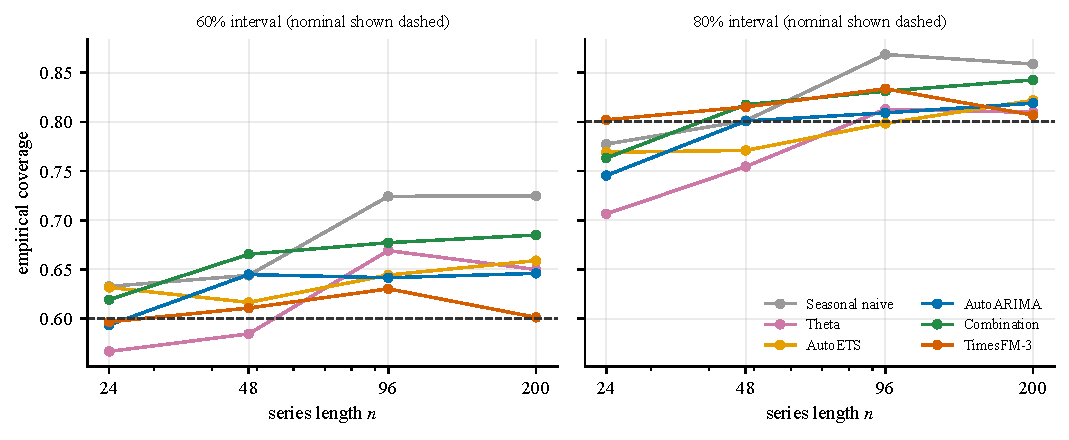
\includegraphics[width=\textwidth]{../figures/fig3_coverage.pdf}
\caption{Empirical coverage of the nominal 60\% and 80\% intervals, averaged over all nine
processes, against series length. The nominal level is dashed. TimesFM-3's 80\% coverage stays
within 0.802--0.834 across every length; the classical methods under-cover at $n = 24$ and
over-cover from $n = 96$.}
\label{fig:coverage}
\end{figure}

Averaged over the processes (\figureref{fig:coverage}), TimesFM-3's 80\% coverage stays between 0.802 and
0.834 at every length, on average across lengths closer to nominal than any other method, and it does not
deteriorate with the horizon (0.786 at $h = 1$, 0.814 over $h = 1$--12). Averaging lets over- and
under-coverage cancel, however; the mean per-cell absolute deviation from nominal is 0.047 for TimesFM-3,
0.066 for AutoARIMA, 0.089 for the combination, 0.101 for AutoETS, 0.127 for Theta and 0.144 for seasonal
naive, and TimesFM-3's per-cell 80\% coverage ranges from 0.583 to 0.921. No method delivers reliable 80\%
intervals on all nine processes. The classical intervals rest on Gaussian innovations, violated by
construction on D8 (Bernoulli occurrence with Poisson sizes) and D9 (conditionally Gaussian but
unconditionally heavy-tailed errors). An interval score, which rewards narrow intervals and penalises
outcomes outside them (80\% interval, scaled as MSIS), puts TimesFM-3 first in 22 of the 36 cells
(Supporting Information, Table~S12). On the structural break D6 every classical method covers 0.966 to
0.999, because the break inflates the estimated variance and the intervals become very wide (scaled widths
4.8 to 10.4); TimesFM-3 covers 0.828 to 0.889 with intervals about half as wide (3.0 to 5.1) and has the
lowest interval score at every length.

TimesFM-3 beats the pre-registered mean combination in 27 of 30 significant comparisons. Because the mean
is not robust to a failing member such as Theta, a \emph{median} combination of the same three methods was
also tried (post hoc), in the spirit of \citet{petropoulos2020scum}; it is slightly worse (mean MASE 1.712
against 1.656, TimesFM-3 1.439), and TimesFM-3 still wins 25 of 29 significant comparisons. Under absolute
error the mean combination can never be worse than the average of its members, by convexity, a guarantee
the median does not carry.

\section{Extended evaluation}
\label{sec:extended}

This section asks how precise the summaries of \sectionref{sec:results} are (\sectionref{sec:mcse}),
whether stronger benchmarks and other foundation models change them (\sectionref{sec:benchmarks}), how
much they depend on the configuration of TimesFM-3 (\sectionref{sec:tfm-check}), and what the
intermittent-demand result means once simple benchmarks are included (\sectionref{sec:d8-extended}),
and what changes at a longer horizon (\sectionref{sec:horizon48}). All of it is post hoc.

\subsection{Monte Carlo uncertainty}
\label{sec:mcse}

The Monte Carlo standard error of a cell's mean MASE is 1.5\% to 6.2\% of the mean (median 3.2\%;
Supporting Information, Table~S2). Bootstrapping the replications within each cell (2\,000 draws, paired
across methods), the worst ratio of TimesFM-3 to the cell-best method is 1.31 (95\% interval 1.28 to 1.36)
and that of AutoARIMA, the smallest among the classical methods, 2.22 (2.07 to 2.38); their difference has
an interval of 0.75 to 1.05. Because the best method of a cell is chosen on the same replications, the
statistic could be biased upwards; choosing it on one half of the replications and estimating the ratio on
the other gives 1.32, so the bias is small. These intervals reflect Monte Carlo error only, not the choice
of processes and parameters, which \sectionref{sec:robustness} varies. The count of cells won is less
stable---TimesFM-3's 16 has an interval of 13 to 20---and no conclusion rests on it.

\subsection{Stronger classical benchmarks and other foundation models}
\label{sec:benchmarks}

Six methods were added (\tableref{tab:extended}): dynamic optimised Theta \citep[DOTM;][]{fiorucci2016dotm};
the Comb benchmark of M4, the mean of simple, Holt and damped exponential smoothing on seasonally adjusted
data \citep{makridakis2020m4}; a combination of AutoETS, AutoARIMA and DOTM; TimesFM-2.5
\citep{timesfm25card} and Chronos-Bolt (Base, 205 million parameters) \citep{ansari2024chronos,
chronosboltcard}, both zero-shot and Apache-2.0 licensed; and TimesFM-3 with its developers' evaluator
settings (\sectionref{sec:tfm-check}). TimesFM-2.5 was run with the same evaluator settings (symmetric
averaging, positivity, quantile-crossing correction) and a context limit of 512 points, which truncates no
simulated series, so its matched comparison is with the evaluator-settings row of TimesFM-3; Chronos-Bolt
was run with its defaults. Three further configurations were added afterwards: Chronos-2
\citep{ansari2025chronos2} and TiRex \citep{auer2025tirex}, two newer zero-shot models with 120 and 35 million
parameters, both run with their package defaults, and TimesFM-2.5 with flip invariance and positivity
switched off, which matches the default settings of the main TimesFM-3 runs.

\begin{table}[!htbp]
\centering
\begin{threeparttable}
\caption{Robustness of fifteen methods across the 36 cells of the main design.}
\label{tab:extended}
\small\setlength{\tabcolsep}{4pt}
\begin{tabular}{lcccc}
\toprule
Method & Worst ratio to best & Mean ratio to best & Within 10\% (\%) & Cells won \\
\midrule
TimesFM-3, evaluator settings & 1.27 [1.26, 1.33] & 1.058 [1.055, 1.066] & 81 & 5 [2, 8] \\
TimesFM-3 & 1.31 [1.29, 1.36] & 1.063 [1.060, 1.072] & 78 & 0 [0, 4] \\
TimesFM-2.5 & 2.18 [2.04, 2.33] & 1.121 [1.116, 1.130] & 67 & 7 [2, 8] \\
TiRex & 2.24 [2.06, 2.45] & 1.121 [1.116, 1.131] & 64 & 0 [0, 4] \\
TimesFM-2.5, settings off & 2.26 [2.10, 2.44] & 1.124 [1.120, 1.134] & 67 & 3 [0, 5] \\
AutoARIMA & 2.22 [2.08, 2.39] & 1.131 [1.125, 1.142] & 64 & 8 [5, 10] \\
Chronos-2 & 2.75 [2.56, 2.97] & 1.139 [1.135, 1.150] & 67 & 4 [3, 6] \\
Combination (ETS, ARIMA, DOTM) & 2.99 [2.84, 3.16] & 1.241 [1.236, 1.253] & 47 & 1 [0, 2] \\
Combination (Theta, ETS, ARIMA) & 3.00 [2.85, 3.17] & 1.243 [1.237, 1.255] & 44 & 1 [1, 3] \\
Chronos-Bolt & 3.06 [2.95, 3.25] & 1.296 [1.291, 1.309] & 58 & 1 [0, 2] \\
AutoETS & 3.50 [3.28, 3.73] & 1.312 [1.304, 1.327] & 31 & 1 [0, 2] \\
Seasonal naive & 5.70 [5.47, 6.03] & 1.347 [1.337, 1.362] & 25 & 2 [1, 3] \\
DOTM & 4.66 [4.34, 4.99] & 1.413 [1.405, 1.429] & 22 & 1 [1, 2] \\
M4 Comb & 4.45 [4.18, 4.79] & 1.456 [1.447, 1.474] & 19 & 1 [0, 2] \\
Theta & 4.69 [4.37, 5.03] & 1.476 [1.467, 1.493] & 19 & 1 [1, 2] \\
\bottomrule
\end{tabular}
\begin{tablenotes}[flushleft]\footnotesize
\item \textit{Note:} Main design, 7\,200 series, mean MASE over $h = 1, \dots, 12$, ratios to the best of the fifteen methods in each of the 36 (process, length) cells. Brackets: 95\% intervals from 500 bootstrap resamples of the replications within each cell. Mean ratio is the geometric mean over cells. Among the original six methods alone, the worst ratio of TimesFM-3 is 1.31 [1.28, 1.36] and that of AutoARIMA 2.22 [2.05, 2.38].
\end{tablenotes}
\end{threeparttable}
\end{table}


The stronger classical benchmarks do not change the picture. DOTM and the Comb benchmark share Theta's
failure on D4, where a classical decomposition with fixed seasonal indices meets a seasonal pattern that
evolves, and replacing Theta by DOTM leaves the combination's worst ratio at 2.99. TimesFM-3 wins 28 of 29
significant comparisons against DOTM and all 29 against the Comb benchmark; AutoARIMA remains the only
classical method it does not clearly beat (11 wins to 9). \textbf{Among the five foundation models,
the robustness belongs to TimesFM-3 alone} (\tableref{tab:extended}): TimesFM-2.5 has a
worst ratio of 2.18 (on D7 at $n = 24$), and 2.26 with its settings switched off, so the difference is not one
of configuration; TiRex has 2.24, Chronos-2 2.75 (on D6 at $n = 24$) and Chronos-Bolt 3.06, against 2.22 for
AutoARIMA. In the median cell every foundation model but Chronos-Bolt is within 2\% to 4\% of the best, and TimesFM-2.5 is the best method in
7 cells, more than any model but AutoARIMA (8). Like TimesFM-3, the newer models do not clearly beat AutoARIMA
(Chronos-2 10--10, TiRex 9--12). Friedman tests with Nemenyi critical differences \citep{demsar2006statistical}
within each regime agree with the pairwise tests: TimesFM-3 is tied for the best mean rank on the linear
processes (with TimesFM-2.5, TiRex and AutoARIMA) and on the break and saturation processes (with no other
method), and AutoARIMA has the best mean rank on the seasonal processes, tied only with TimesFM-3 under its
evaluator settings. Averaged over the design, the 80\% intervals of TimesFM-3 cover 0.814 (Monte Carlo SE
0.003), TimesFM-2.5 0.812, Chronos-2 0.789, TiRex 0.842, Chronos-Bolt 0.834 and AutoARIMA 0.794 (Supporting Information, Table~S3, by process for the models of the
first comparison).

\subsection{Configuration and output of TimesFM-3}
\label{sec:tfm-check}

The developers' benchmark evaluator averages the forecasts of a series and its negation and constrains
non-negative series to non-negative forecasts, whereas the main study used the package defaults. With
the evaluator settings the worst ratio falls from 1.31 to 1.27 and the geometric mean ratio over the twelve
methods from 1.059 to 1.054; no conclusion changes. The output is a $12 \times 9$ array of deciles whose raw
median equals the point forecast exactly; quantile crossing occurs in 32\% to 46\% of steps on D8 and
essentially never elsewhere, so only on D8 does it matter that the main runs take the raw median as point
forecast and the evaluator-settings runs the median after sorting. Given the month of the year as
past-and-future covariates ($\sin 2\pi t/12$, $\cos 2\pi t/12$) on D4 and D5---the information the classical
methods receive through their period---TimesFM-3's mean MASE rises in seven of the eight cells (for example
1.124 to 1.194 on D4 at $n = 96$), so supplying the period in this form did not close AutoARIMA's seasonal
advantage. Using the mean of the deciles instead of the median as point forecast changes no process by more
than 0.01 except D6 (0.835 to 0.875) and D8.

\subsection{Intermittent demand re-examined}
\label{sec:d8-extended}

Because MASE rewards the conditional median, which on D8 is near zero, the trivial all-zero forecast
belongs in the comparison, and because D8 is independent over time, so do benchmarks that simply use the
empirical distribution of the history \citep{willemain2004bootstrap}: its mean as point forecast and its
deciles as predictive distribution. \tableref{tab:d8ext} adds them, with the scaled mean error (bias) and
periods in stock \citep[PIS;][]{wallstrom2010pis}, which accumulates forecast errors as a stock position
would.

\begin{table}[!htbp]
\centering
\begin{threeparttable}
\caption{Intermittent demand (D8) re-examined with simple benchmarks, bias and stock measures.}
\label{tab:d8ext}
\small\setlength{\tabcolsep}{4pt}
\begin{tabular}{lccccc}
\toprule
Method & MASE & RMSSE & sME & sPIS & SPL \\
\midrule
All-zero forecast & 0.668--0.718 & 0.785--0.825 & $-0.72$ to $-0.67$ & $-91$ to $-81$ & -- \\
History: mean; empirical deciles & 0.924--0.975 & 0.692--0.744 & $-0.07$ to $-0.02$ & $-13$ to $-3$ & 0.282--0.314 \\
TimesFM-3 & 0.683--0.780 & 0.774--0.806 & $-0.67$ to $-0.57$ & $-81$ to $-74$ & 0.288--0.325 \\
TimesFM-3, mean of deciles & 0.915--1.002 & 0.694--0.760 & $-0.06$ to $-0.01$ & $-10$ to $-4$ & 0.288--0.325 \\
TimesFM-2.5 & 0.678--0.770 & 0.777--0.806 & $-0.67$ to $-0.59$ & $-81$ to $-74$ & 0.289--0.324 \\
Chronos-Bolt & 0.708--0.786 & 0.758--0.789 & $-0.59$ to $-0.54$ & $-72$ to $-65$ & 0.294--0.328 \\
Chronos-2 & 0.681--0.750 & 0.776--0.808 & $-0.66$ to $-0.63$ & $-81$ to $-76$ & 0.290--0.323 \\
TiRex & 0.683--0.776 & 0.771--0.800 & $-0.67$ to $-0.58$ & $-81$ to $-73$ & 0.289--0.324 \\
Croston--SBA & 0.921--1.025 & 0.694--0.763 & $-0.04$ to $0.05$ & $-7$ to $2$ & -- \\
ADIDA & 0.926--0.972 & 0.700--0.753 & $-0.09$ to $-0.02$ & $-16$ to $-5$ & -- \\
TSB & 0.916--0.971 & 0.716--0.764 & $-0.10$ to $0.00$ & $-17$ to $-1$ & -- \\
AutoARIMA & 0.924--0.996 & 0.698--0.765 & $-0.05$ to $-0.03$ & $-12$ to $-3$ & 0.341--0.380 \\
\bottomrule
\end{tabular}
\begin{tablenotes}[flushleft]\footnotesize
\item \textit{Note:} Process D8, 200 replications per length; ranges over the four lengths $n \in \{24, 48, 96, 200\}$. sME: mean error (forecast minus actual) scaled by the MASE denominator; negative values mean under-forecasting. sPIS: periods in stock \citep{wallstrom2010pis}, cumulated over the horizon and scaled by the mean demand of the context; large negative values mean persistent stock-outs. SPL: scaled pinball loss over the nine deciles, defined only for methods with a predictive distribution. TimesFM-3, mean of deciles, uses the average of its nine deciles as point forecast. History: the mean of the context as point forecast and the empirical deciles of the context as predictive distribution; the median of the context is zero or near it, so its point forecast would repeat the all-zero row.
\end{tablenotes}
\end{threeparttable}
\end{table}


\textbf{The all-zero forecast has the lowest MASE at every length} (0.668 to 0.718), below TimesFM-3's
median forecast (0.683 to 0.780). The MASE advantage of \sectionref{sec:regimes} is thus the advantage of
a forecast close to zero: its bias ($-0.67$ to $-0.57$ MASE units) and PIS ($-81$ to $-74$) are close to
those of the all-zero forecast and imply persistent stock-outs, so it is not evidence of useful accuracy.
With the mean of its deciles as point forecast, TimesFM-3 has an RMSSE of 0.694 to 0.760 and a bias within
0.06 of zero, level with the best Croston-family method and with the mean of the history (0.692 to 0.744).
Its pinball loss, 0.288 to 0.325, is about 15\% below that of the classical methods (0.341 to 0.380), but
their quantiles come from Gaussian intervals that put probability on negative demand; the empirical deciles
of the history score 0.282 to 0.314, slightly lower than TimesFM-3 at every length. \textbf{On intermittent
demand, therefore, TimesFM-3 shows no advantage over simple benchmarks}: it behaves much like the empirical
distribution of the history, and its advantage over the classical methods reflects their Gaussian
intervals. The other foundation models, Chronos-2 and TiRex included, behave the same way
(\tableref{tab:d8ext}). The result concerns a process that is independent over time, the case most favourable
to history-based benchmarks.

\subsection{A longer horizon}
\label{sec:horizon48}

Calibration of foundation models is reported to degrade with the horizon \citep{adler2026calibrated}, and the
main design stops at 12 steps. The nine processes were therefore regenerated with the same seeds for a
48-step horizon and forecast by the six pre-registered methods, TimesFM-2.5 and Chronos-2 (Supporting
Information, Section~S7 and Figure~S3). Because the inflection of D7 sits at $0.6(n + H)$, the longer horizon
moves it into the context for $n = 200$, so that the series has already flattened when the forecast starts.
Over the first 12 steps the picture of \sectionref{sec:results} is recovered: without D7, TimesFM-3's worst
ratio to the best method is 1.31 and AutoARIMA's 2.11. Further out it is not. Over steps 25 to 48,
\textbf{AutoARIMA has the smaller worst case} (1.41 against 1.80, D7 excluded), although TimesFM-3 remains
closer to the best method in the median cell (1.075 against 1.109). On D7 at $n = 200$ every foundation model
forecasts a decline while the process stays at its plateau near 200: TimesFM-3's mean forecast falls to 128
by step 48, TimesFM-2.5's to 98 and Chronos-2's to 146, and their mean MASE over the 48 steps is 8.37, 12.22
and 5.30, against 1.11 for seasonal naive and 2.51 for AutoARIMA. What in the models produces the decline
cannot be established here. The coverage of TimesFM-3's 80\% intervals falls from 0.788 over steps 1 to 12 to
0.760 over steps 25 to 48, and AutoARIMA's from 0.760 to 0.720, so both drift away from nominal, as
\citet{adler2026calibrated} report for foundation models. The robustness of \sectionref{sec:estimability} is
thus a property of short horizons.

\section{Representativeness and robustness of the design}
\label{sec:robustness}

Simulation conclusions are conditional on the processes and parameters used. This section asks how
closely the simulated series resemble real ones (\sectionref{sec:representativeness}) and whether the
conclusions survive random parameters and departures from the assumptions (\sectionref{sec:departures}).
Both analyses are post hoc.

\subsection{Representativeness of the simulated series}
\label{sec:representativeness}

Following \citet{kang2017instance}, each series is summarised by four features: normalised spectral
entropy (forecastability), STL trend strength, STL seasonal strength (period 12) and the first
autocorrelation of the first differences. The simulated series at $n = 96$ and the 1\,000 M4 Monthly
series of \sectionref{sec:realdata}, each cut to the last 96 observations of its training period, are
placed in this space with the features standardised on the M4 series. An M4 series is \emph{covered} when
some simulated series lies at least as close to it as the 95th percentile of the distance from an M4
series to its nearest other M4 series.

\begin{figure}[!htbp]
\centering
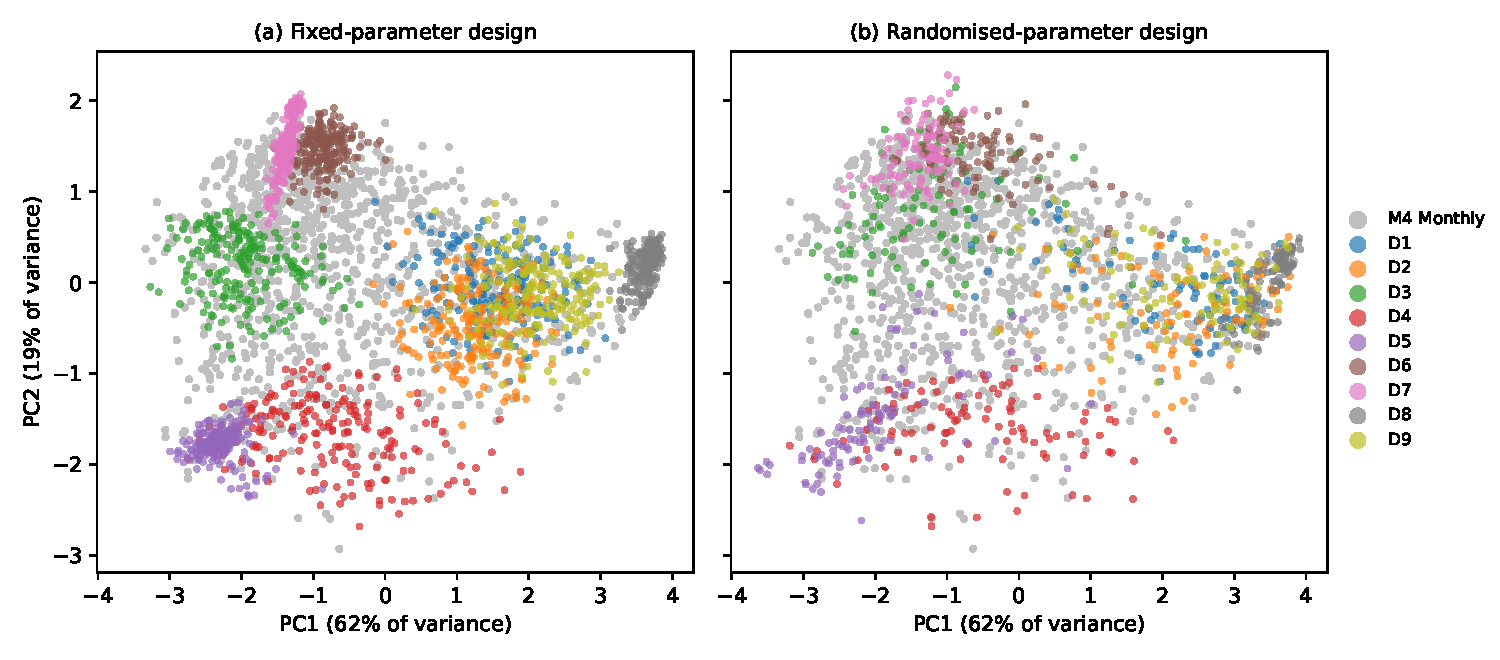
\includegraphics[width=\textwidth]{../figures/fig11_instance_space.pdf}
\caption{Simulated and M4 Monthly series in a four-feature instance space (spectral entropy,
trend strength, seasonal strength and first-order autocorrelation of the differences), first two
principal components. Grey points are M4 series; coloured points are simulated series at
$n = 96$. (a) The fixed-parameter design covers 48.5\% of the M4 series; (b) the randomised-parameter
design covers 75.8\%, with coverage defined in \sectionref{sec:representativeness}.}
\label{fig:instance}
\end{figure}

The fixed design covers 48.5\% of the M4 series (bootstrap interval 45.2\% to 51.4\%;
\figureref{fig:instance}): each process forms a compact cluster and the regions between them, which hold
many real series, are empty. The randomised design of \sectionref{sec:departures} covers 75.8\% (73.2\% to
78.4\%). Across thresholds from the 80th to the 99th percentile, lengths of 48,
96 and 200, and a six-feature space adding the first autocorrelation and lumpiness, the randomised design
covers 76\% to 89\% of M4 at the 95th percentile and never less than the fixed design, also when the latter
is subsampled to equal size; conversely, 60\% to 92\% of the randomised series lie within the same distance
of some M4 series, fewest at $n = 200$. The parameter ranges were set before this statistic was first
computed. M4 series are more strongly trending than the simulated ones (median trend strength 0.87 against
0.63), and only 1.5\% lie nearest to D8, because M4 has no intermittent series; the intermittent-demand
results rest on the simulation alone.

\subsection{Randomised parameters and departures from the assumptions}
\label{sec:departures}

Every series now draws its own parameters uniformly from wide ranges containing the fixed values of
\tableref{tab:dgps} (Supporting Information, Table~S8): autoregressive coefficients up to 0.95,
intermittency from lumpy ($p = 0.1$) to nearly continuous ($p = 0.6$), breaks of three to fifteen noise
standard deviations in either direction. Four versions use the same 7\,200 parameter draws (200 per process
and length): \emph{random parameters} with Gaussian innovations; \emph{heavy tails}, Student-$t_3$
innovations of the same variance built from the same normal draws (negative binomial sizes on D8);
\emph{outliers}, each context point shifted with probability 0.03 by four to six robust standard deviations
(a demand multiplied by five on D8), with the held-out values left clean; and \emph{tested seasonality},
in which the classical methods use $m = 12$ only if the 90\% autocorrelation test of the M4 benchmarks
\citep{makridakis2020m4} finds seasonality, applied when at least three cycles are observed, and
$m = 1$ otherwise. TimesFM-3 never
receives a period, so its forecasts are unchanged in the last version.

\begin{table}[!htbp]
\centering
\begin{threeparttable}
\caption{Headline conclusions under randomised parameters and departures from the assumptions.}
\label{tab:robust-design}
\small\setlength{\tabcolsep}{4pt}
\begin{tabular}{lcccc}
\toprule
 & Random & Heavy tails & Outliers & Tested seas. \\
\midrule
TimesFM-3 cell wins (of 36) & 14 & 15 & 16 & 16 \\
TimesFM-3 median ratio to cell-best & 1.029 & 1.038 & 1.004 & 1.017 \\
TimesFM-3 worst ratio to cell-best & 1.56 & 1.54 & 1.49 & 1.55 \\
Smallest worst ratio, classical & 2.12 & 2.32 & 2.09 & 1.58 \\
Significant comparisons, won--lost & 93--29 & 100--28 & 101--27 & 100--27 \\
D4, $n \geq 48$: AutoARIMA better (of 3) & 3 & 3 & 2 & 3 \\
D8: Croston better on RMSSE (of 4) & 4 & 4 & 4 & 4 \\
D5, $n = 24$: AutoETS / seasonal naive ($m = 12$) & 2.03 & 2.05 & 1.91 & 2.25 \\
\bottomrule
\end{tabular}
\begin{tablenotes}[flushleft]\footnotesize
\item \textit{Note:} 200 replications per (process, length) cell, 7\,200 series per column; every series draws its own parameters from the ranges in Table~S8 of the Supporting Information. Ratios use mean MASE over $h = 1, \dots, 12$. Significant comparisons are paired Wilcoxon tests of TimesFM-3 against each of the five general-purpose classical methods in each cell (180 per column), Benjamini--Hochberg at 0.05 within each (column, opponent) family of 36 cells (the main design's families also include the three horizon slices). The D8 row compares TimesFM-3 with the best of Croston-SBA, TSB and ADIDA; the last row divides by seasonal naive with the true period in every column. In the tested-seasonality column the classical methods use $m = 12$ only where the M4 seasonality test finds seasonality; TimesFM-3's forecasts are those of the first column.
\end{tablenotes}
\end{threeparttable}
\end{table}


In the three versions with a known period the conclusions were qualitatively consistent with the main
design (\tableref{tab:robust-design}), although TimesFM-3's worst ratio lies outside the main design's
bootstrap interval. TimesFM-3 is the best method in 14 to 16 cells and within 4\% of the best in the median
cell; its worst ratio rises to 1.49 to 1.56 (bootstrap intervals up to about 1.75), always on the logistic
process D7 at $n = 96$, while the smallest classical worst ratio is 2.09 to 2.32. With the
Benjamini--Hochberg family per opponent, TimesFM-3 wins 93 to 101 of 180 comparisons and loses 27 to 29,
AutoARIMA again being the opponent it does not clearly beat (7--7, 6--7, 10--4 and 8--6 across the four
versions). AutoARIMA's advantage on D4 with at least four cycles persists (median over the three lengths 21\%
to 26\%; with outliers it is ahead at two of the three lengths, by 15\% and 5\%), and the Croston family keeps
the lower RMSSE on D8 in every version.

\textbf{When the classical methods test for seasonality, the gap in worst ratios closes, but not because they
forecast better}: their smallest worst ratio is 1.58 (1.48 to 1.67, AutoARIMA), level with TimesFM-3's 1.55
(1.41 to 1.71). AutoARIMA's worst cell is still D4 at $n = 24$, and its mean MASE there is unchanged (2.30);
what changes is the yardstick. At $n = 24$ the test cannot be applied, every series is treated as
non-seasonal, and seasonal naive loses the true period that made it the best method in that cell (mean MASE
4.26 instead of 1.09), so TimesFM-3 (1.45) becomes the cell-best. Much of the classical deficit in worst
ratios is thus measured against seasonal naive with a known period. With two cycles the automatic classical
methods recover the seasonality in neither configuration: non-seasonal AutoETS has a mean MASE of 2.55 on D5
and 4.25 on D4, against 1.13 and 1.09 for seasonal naive with the true period and 1.11 and 1.45 for
TimesFM-3.

A response-surface regression of the per-series $\log_2$ ratio of TimesFM-3's MASE to AutoARIMA's on the
standardised parameters, $\log_2 n$ and the version, with standard errors clustered by parameter draw
(Supporting Information, Tables~S4 and~S5, and Figure~S2), shows that the dependence on the settings is
modest. The largest systematic effect is length: each doubling of $n$ moves the ratio against TimesFM-3 by
20\% on D4 and 11\% on D5, and in its favour on D6 and D8. Outliers favour TimesFM-3 on the seasonal
processes (14\% and 10\%); the other version effects are at most 0.09 in absolute value. Among the
parameters only the demand probability of D8 has a large effect; the ratio is flat in the autoregressive
coefficient of D1 and the GARCH persistence of D9, grows in favour of TimesFM-3 with the size of the break in
D6, and varies with the inflection point of D7 in a way a linear term does not capture (Figure~S2). The
regressions explain little of the per-series variation ($R^2 \leq 0.26$).

\section{Application to M4 monthly data}
\label{sec:realdata}

Whether TimesFM-3 has seen the M4 data cannot be settled, but the documented corpus makes it less likely
than for many public benchmarks: its real-world part is the GIFT-Eval pre-training collection (without the
datasets overlapping fev-bench), Wikipedia page views and Google Trends \citep{timesfm3card}, and that
collection is built to exclude the GIFT-Eval test datasets, of which M4 Monthly is one
\citep{aksu2024gifteval, giftevalpretrain}. The exclusion works at the level of datasets, and the
synthetic and augmented part of the corpus is not documented. TimesFM-2.5 lists the same sources
\citep{timesfm25card}. The position of Chronos-Bolt differs: the original Chronos models were trained on M4
Monthly with its final 18 observations, the official test period, held out \citep[Table~2]{ansari2024chronos};
if, as its model card suggests, Chronos-Bolt shares that corpus, its M4 forecasts are in-domain rather than
zero-shot. The corpora of Chronos-2 and TiRex were not checked for M4, and their M4 results are read in the
same way. Because no corpus can be inspected, the real-data tier is secondary evidence. This section reports
a rolling-origin evaluation (\sectionref{sec:m4results}), the official M4 test period
(\sectionref{sec:m4official}) and an experiment with truncated histories (\sectionref{sec:truncation}); the
last two are post hoc.

\subsection{Rolling-origin evaluation}
\label{sec:m4results}

A seeded sample of 1\,000 series is drawn from the 32\,581 M4 Monthly series with at least 138 training
observations, enough for a context of 120 and the 18-month horizon. Their training periods have a median of 281 observations (interquartile range 198
to 306), against 202 (82 to 306) for all 48\,000 series, so the sample over-represents the long end of the
population. Each series is evaluated at up to three origins 12 months apart with M4's horizon $h = 18$
(2\,932 windows; the shortest series cannot support a third origin); consecutive windows overlap by six
months, so the errors of a series are averaged over its origins and the series are the independent units of
the paired Wilcoxon tests. TimesFM-3 and the pre-registered classical methods were run on this tier.
TimesFM-3 (mean MASE 0.914) significantly outperforms seasonal naive (1.280; better on 80.1\% of series),
Theta (0.970; 56.8\%) and AutoETS (0.951; 54.1\%), and shows no detectable difference from AutoARIMA (0.923;
52.6\%, adjusted $p = 0.27$) or the combination (0.907; 48.5\%, adjusted $p = 0.27$).

This ties TimesFM-3 with AutoARIMA on long, mostly seasonal series, rather than showing the 21\% to 24\%
AutoARIMA advantage found on the simulated D4. The simulated seasonal process is a single, sharply seasonal
model, whereas real series mix trend, seasonality and irregular components in proportions the simulation
does not reproduce (\sectionref{sec:representativeness}); an advantage from contamination cannot be excluded
either. The probabilistic results also diverge: TimesFM-3's 80\% intervals cover 0.765 against 0.801 for the
combination, yet its pinball loss is the lowest of the six methods (0.363, against 0.365 for the combination
and 0.374 for AutoARIMA). Its distribution is slightly better overall while its 80\% interval is too narrow,
the fragility of foundation-model calibration reported by \citet{adler2026calibrated}.

\subsection{The official M4 test period}
\label{sec:m4official}

Rolling origins cut from the training data cannot be placed against published M4 results, so the same
series were also forecast for the official 18-month test period from their full histories and scored as in
M4, with the overall weighted average (OWA) of sMAPE and MASE relative to the official Naive2 forecasts
\citep{makridakis2020m4}. The comparison includes the methods of \sectionref{sec:benchmarks} and, post hoc,
the published point forecasts of the ten best M4 submissions, among them the winning hybrid of exponential
smoothing and a recurrent network \citep{smyl2020hybrid} and the feature-based combination FFORMA
\citep{monteromanso2020fforma}; scored on all 48\,000 monthly series, the downloaded files reproduce the
published M4 results.

\begin{table}[!htbp]
\centering
\begin{threeparttable}
\caption{M4 Monthly official test period: accuracy, OWA and multiple comparisons.}
\label{tab:m4official}
\small\setlength{\tabcolsep}{4pt}
\begin{tabular}{lcccccc}
\toprule
Method & sMAPE & MASE & OWA & Coverage & MSIS & Mean rank \\
\midrule
TimesFM-3, evaluator settings & 8.01 & 0.923 & 0.857 & 0.765 & 4.50 & 6.14$^\ast$ \\
TimesFM-3 & 8.05 & 0.929 & 0.862 & 0.761 & 4.54 & 6.25$^\ast$ \\
TimesFM-2.5 & 8.15 & 0.922 & 0.864 & 0.812 & 4.53 & 6.37$^\ast$ \\
Combination (ETS, ARIMA, DOTM) & 8.16 & 0.928 & 0.867 & 0.789 & 4.74 & 6.11$^\ast$ \\
Combination (Theta, ETS, ARIMA) & 8.16 & 0.929 & 0.868 & 0.789 & 4.76 & 6.06$^\ast$ \\
AutoARIMA & 8.50 & 0.939 & 0.891 & 0.779 & 4.91 & 6.45$^\ast$ \\
Chronos-Bolt & 8.40 & 0.971 & 0.900 & 0.800 & 4.70 & 6.91 \\
AutoETS & 8.45 & 0.966 & 0.900 & 0.784 & 4.98 & 6.83 \\
M4 Comb & 8.50 & 0.982 & 0.911 & -- & -- & 7.16 \\
DOTM & 8.59 & 0.996 & 0.922 & 0.728 & 5.27 & 7.39 \\
Theta & 8.59 & 1.006 & 0.926 & 0.723 & 5.36 & 7.37 \\
Naive2 & 9.22 & 1.092 & 1.000 & -- & -- & 8.32 \\
Seasonal naive & 10.39 & 1.306 & 1.161 & 0.780 & 6.56 & 9.66 \\
\bottomrule
\end{tabular}
\begin{tablenotes}[flushleft]\footnotesize
\item \textit{Note:} 1\,000 M4 Monthly series, each forecast for the official 18-month test period from its full training history. sMAPE and MASE as defined in M4; OWA relative to the official Naive2 forecasts. Coverage and MSIS use the nominal 80\% interval, the widest that every probabilistic method can form from nine deciles. Mean rank: average rank of per-series MASE among the 13 methods (Friedman $\chi^2 = 847$, $p < 10^{-100}$); $^\ast$ marks methods whose mean rank is within the Nemenyi critical difference (0.58) of the best.
\end{tablenotes}
\end{threeparttable}
\end{table}


Theta and the Comb benchmark improve on Naive2 by 7\% to 9\% in OWA (\tableref{tab:m4official}), in line
with the competition. \textbf{Four M4 entries are ahead of every foundation model}: FFORMA (OWA 0.831),
Jaganathan and Prakash (0.841), Smyl's hybrid (0.848) and Pawlikowski et al.\ (0.849). TimesFM-3 (0.862;
0.857 with its evaluator settings) is level with the entries ranked fifth to seventh in M4 (0.858 to 0.864),
TiRex (0.855) and Chronos-2 (0.860) are close to it, and the classical combination (0.868) and AutoARIMA
(0.891) follow. On this sample the M4 entries' OWA differs from their published monthly values by up to
0.03, as much as the gaps between them. A Friedman test on per-series ranks, with one configuration per model
and without Naive2 \citep{benavoli2016should}, rejects the equality of the 22 methods, but ten lie within the
Nemenyi critical difference of the best mean rank \citep{demsar2006statistical}: five M4 entries, the
classical combination, TimesFM-3, Chronos-2 and TiRex. On real monthly series with long histories, zero-shot
TimesFM-3 matches good specialised methods of 2018 without per-series tuning, but not the best of them.

\subsection{Truncated histories}
\label{sec:truncation}

The official test period was also forecast from only the last 24, 48 or 96 observations of each training
series, with the full-history MASE denominator so that only the information available to the methods
changes (\tableref{tab:truncation}). The simulation's estimability result reappears: with 24 observations,
where the classical methods again have two cycles for a period of 12, the foundation models lead---TiRex
1.027, TimesFM-3 1.046, TimesFM-2.5 1.050---against 1.096 for the best classical method, the combination,
and 1.175 for AutoARIMA; the difference was not tested. With 48 observations the combination is level with
them (0.955 against 0.952 to 0.972), and with the full history the leading methods are within 2\% of one
another. Truncation also moves the information set away from the full series a model could have been trained
on, although it cannot rule out that the series were seen.

\begin{table}[!htbp]
\centering
\begin{threeparttable}
\caption{M4 Monthly with truncated contexts: mean MASE by context length.}
\label{tab:truncation}
\small\setlength{\tabcolsep}{4pt}
\begin{tabular}{lcccc}
\toprule
Method & Last 24 & Last 48 & Last 96 & Full \\
\midrule
TimesFM-3 & 1.046 & 0.961 & 0.942 & 0.929 \\
TimesFM-3, evaluator settings & 1.045 & 0.960 & 0.936 & 0.923 \\
TimesFM-2.5 & 1.050 & 0.972 & 0.952 & 0.922 \\
Chronos-Bolt & 1.158 & 1.023 & 0.965 & 0.971 \\
Chronos-2 & 1.087 & 0.952 & 0.935 & 0.917 \\
TiRex & 1.027 & 0.956 & 0.949 & 0.916 \\
AutoARIMA & 1.175 & 1.019 & 0.979 & 0.939 \\
AutoETS & 1.129 & 0.996 & 0.995 & 0.966 \\
Theta & 1.150 & 1.011 & 1.003 & 1.006 \\
DOTM & 1.167 & 1.012 & 0.991 & 0.996 \\
Combination (Theta, ETS, ARIMA) & 1.096 & 0.955 & 0.947 & 0.929 \\
Combination (ETS, ARIMA, DOTM) & 1.111 & 0.959 & 0.945 & 0.928 \\
Seasonal naive & 1.306 & 1.306 & 1.306 & 1.306 \\
\bottomrule
\end{tabular}
\begin{tablenotes}[flushleft]\footnotesize
\item \textit{Note:} Mean MASE on the M4 official test period when each method sees only the last 24, 48 or 96 training observations, or the full history (median 281 observations). All columns use the full-history MASE denominator, so only the information given to the methods changes. Seasonal naive uses only the last 12 observations and is unaffected.
\end{tablenotes}
\end{threeparttable}
\end{table}


\section{Operational considerations}
\label{sec:operational}

Accuracy is not the only criterion. This section considers computational cost (\sectionref{sec:cost}) and
licensing, interpretability and the basis of prediction intervals (\sectionref{sec:licence}).

\subsection{Computational cost}
\label{sec:cost}

Timed separately on the same 200 seasonal series of length 96, seasonal naive took 3.1\,ms per series,
Theta 9.0\,ms, TimesFM-3 23.2\,ms (batched on an NVIDIA GTX 1660 Ti, excluding a one-off model load of
3.0\,s), AutoETS 102.0\,ms and AutoARIMA 2\,382.7\,ms, each classical method on one CPU core: automatic
ARIMA searches over orders and fits each candidate by maximum likelihood, separately for every series,
whereas TimesFM-3 amortises one forward pass over a batch. Per series, Theta and seasonal naive were thus
faster than TimesFM-3 and AutoETS about four times slower, and the classical methods parallelise trivially:
in the main run, all four classical methods over the 7\,200 series took 7.3 minutes on 22 cores, against 3.2
minutes for TimesFM-3 on one consumer GPU, a ratio of $2.3\times$ that is dominated by AutoARIMA and depends
on the hardware. Memory cannot be compared directly, because the profiler used sees neither the compiled
kernels of the classical methods nor GPU memory; structurally, the classical methods hold a handful of
parameters per series, whereas TimesFM-3 keeps its checkpoint of about 1.3\,GB resident, whatever the number
of series.

\subsection{Licensing, interpretability and prediction intervals}
\label{sec:licence}

TimesFM-3's weights are released under the TimesFM Non-Commercial License v1.0, which grants use ``solely
for your Non-Commercial Purposes'' and requires a separate licence for any ``commercial or production
activity'' \citep{timesfm3repo, timesfm3card} (accessed 23 September 2026). The source code is Apache-2.0,
as were the weights of TimesFM-2.5 and Chronos-Bolt, but the version-3 weights are not: \textbf{for a
commercial application, TimesFM-3 is not licensed as released}, whatever its accuracy, and the alternatives
are TimesFM-2.5, separate terms or a classical method. Licensing is routinely omitted from model comparisons
although it decides which models an entire class of users may use.

An ARIMA or ETS fit reports its orders, coefficients, smoothing parameters and standard errors, which
support residual diagnostics, tests for remaining structure and an explanation of why a forecast turns
where it does. TimesFM-3 exposes none of this: when it forecasts poorly, there is nothing to inspect. Its
quantiles are learned outputs with no accompanying theory; they were well calibrated on average in the
simulation (\sectionref{sec:coverage}) but under-covered on M4, and their behaviour on a process unlike anything in
the pre-training corpus is unknown. In regulated settings where a forecast must be justified, these
differences may outweigh the accuracy comparison.

\section{Discussion}
\label{sec:discussion}

This section assesses the pre-registered hypotheses (\sectionref{sec:hypotheses}), interprets the balance
between robustness and peak accuracy (\sectionref{sec:tradeoff}), gives practical recommendations
(\sectionref{sec:recommendations}) and states the limitations (\sectionref{sec:limitations}).

\subsection{Assessment of the pre-registered hypotheses}
\label{sec:hypotheses}

\textbf{None of the five hypotheses survives unqualified}: H1 and H5 are not supported, H4 is contradicted,
and H2 and H3 are partially supported. The protocol did not state decision rules, so these verdicts are
judgements on the pattern of pre-registered tests. \textbf{H1} (correctly specified classical models beat
TimesFM-3 on their home ground, most at short lengths) is not supported as stated---at short lengths the gap
runs the other way---and holds only where a model is both correctly specified and estimable (D4 and D5 at
$n \geq 48$). \textbf{H2} (TimesFM-3 wins wherever no classical form is correct) is partially supported:
mildly on breaks; not on the logistic process, where the outcome depends on length; and on intermittent
demand only against the classical methods, not against simple benchmarks built from the history.
\textbf{H3} (on D9 the families tie in the mean and classical intervals under-cover) is partially supported:
they tie, but only AutoARIMA under-covers. \textbf{H4} (the combination beats every classical method and is
TimesFM-3's hardest opponent) is contradicted in both clauses: AutoARIMA beats the combination on mean MASE
and is the harder opponent (11--9 against 27--3). \textbf{H5} (both families under-cover at 80\%, TimesFM-3
more at longer horizons) is not supported: averaged over processes TimesFM-3 is close to nominal, its
coverage does not fall with the horizon, and the classical methods over-cover from $n = 96$; per cell the
deviations are large but not systematically downward.

\subsection{Robustness versus peak accuracy}
\label{sec:tradeoff}

The classical methods' 20 cell wins are spread over five methods, so which classical method wins is not
knowable in advance without the model selection a foundation model is meant to remove. TimesFM-3, one
untuned model, is not significantly worse than the best classical method in 25 of the 36 cells; the best
classical method is ahead in the other 11, over five processes, by small margins on D2 and D3 and by large
ones only on D4, D5 and D7 at $n = 96$ (these comparisons with a selected opponent are descriptive). The
evidence therefore supports neither the conclusion that foundation models have superseded classical methods
nor the opposite, but a narrower one: \textbf{in this design TimesFM-3 behaved robustly rather than with peak
accuracy}. It is rarely the best method and never among the worst, whereas the automatic classical methods
are sometimes excellent and sometimes catastrophic. For one well-understood series that trade is
unattractive; for many heterogeneous series and no capacity to diagnose each one, it favoured TimesFM-3 here.

The extended evidence qualifies the trade four times. Among the foundation models evaluated it belongs to
TimesFM-3 alone (\sectionref{sec:benchmarks}). It holds for short horizons only: at 48 steps AutoARIMA has the
smaller worst case, and every foundation model mistakes a plateau for a decline (\sectionref{sec:horizon48}). Its size depends on the yardstick: much of the classical
deficit is measured against seasonal naive with a known period, and without the two-cycle cells AutoARIMA's
worst ratio is 1.62 against TimesFM-3's 1.31 (\sectionref{sec:estimability}, \sectionref{sec:departures}).
And on the M4 test period with long histories, TimesFM-3 is level with good but not the best M4 entries
(\sectionref{sec:m4official}).

\subsection{Practical recommendations}
\label{sec:recommendations}

The recommendations below are conditional on the processes, lengths and horizon examined. They describe how
the methods behaved here and are offered as diagnostic starting points to be checked on the user's own
data, not as rules; several rest on considerations outside the accuracy comparison, and where the evidence
does not favour one family, more than one option is named.

\textbf{Many heterogeneous series without per-series tuning.} This is where TimesFM-3's robustness mattered
most in this design: it won most significant comparisons against every classical method except AutoARIMA
and was never far from the best method of a cell. Where a model can be identified for a single series, the
classical route loses little---against AutoARIMA the comparisons split 11--9---and keeps parameters,
diagnostics and interval theory that can be explained and audited.

\textbf{Seasonal series.} With at least four observed cycles, AutoARIMA was 21--24\% more accurate than
TimesFM-3 on the seasonal ARIMA process D4 and 4--12\% on the ETS process D5, and seasonal naive was also
ahead on D4. With two cycles the automatic classical methods fell back to non-seasonal models and failed,
and seasonal naive, or TimesFM-3, was the safer choice.

\textbf{Intermittent demand.} Simple benchmarks built from the history were as good as anything tested:
the empirical deciles of the history gave the lowest pinball loss, and its mean, like the Croston family,
the lowest RMSSE. TimesFM-3 came close on both only with a suitable read-out of its deciles, and its median
forecast was no better than forecasting zero. These results come from a process that is independent over
time, the case most favourable to history-based benchmarks.

\textbf{Long horizons.} Beyond about a year of monthly steps the evidence turns: AutoARIMA had the smaller
worst case, and every foundation model forecast a decline on a process that had levelled off, so long-horizon
forecasts from these models should be checked against the recent level before use.

\textbf{Intervals, cost and licence.} TimesFM-3 had the best 80\% interval score in 22 of the 36 cells,
including every length after a structural break (D6); on M4, however, its 80\% intervals under-covered
(0.765 against 0.801 for the classical combination on the rolling origins), so interval quality on real
data should be checked rather than assumed. On the hardware used, TimesFM-3 on a GPU was faster end to end
than the parallelised classical suite, a comparison dominated by AutoARIMA. For commercial deployment the
licence decides before accuracy does: TimesFM-3's weights are non-commercial, and the Apache-2.0
TimesFM-2.5 was less robust in the simulation (worst ratio 2.18) though level with TimesFM-3 on M4.

\subsection{Limitations}
\label{sec:limitations}

First, simulated series are clean and free of the measurement error, calendar effects and regime changes of
applied work; the M4 tier addresses this only in part, and the randomised design still leaves about a
quarter of M4 monthly series, and all other frequencies, outside the regions studied, with coverage in four
features a necessary rather than sufficient condition for similarity. Second, the nine process families are
fixed, the pre-registered horizon is short ($H = 12$) and the longer one was examined in one secondary check,
the seasonal period is 12, and the departures from the assumptions were applied one at a time, so their
interactions were not examined. Third, TimesFM-3 was used zero-shot and
univariate, leaving its multivariate and covariate capabilities untested; fine-tuning was excluded because
fine-tuning on one series of 24 to 200 points is not meaningful for a model of this size and fine-tuning on
the DGPs would remove the separation between model and test data. Fourth, no method was tuned by hand, and
the classical methods were run in \pkg{StatsForecast} at its defaults; a cross-check with \pkg{forecast} on the
seasonal processes reproduced the failures but found one implementation failure, and an expert who identified
each process could select better models. Fifth, five foundation
models were evaluated and they behave differently, so conclusions about one do not transfer to the class;
masked-encoder models such as Moirai \citep{woo2024moirai} were not included. Sixth, the summaries that carry the robustness finding---worst
ratios and win counts---were defined after the protocol and depend on the methods and cells compared.
Seventh, the protocol was frozen before any forecast but held in the replication archive rather than
deposited with an external registry, and several analyses are post hoc---the Croston and history
benchmarks, the combination rule, the Oracle ARIMA, Sections~\ref{sec:extended} and~\ref{sec:robustness},
and the official-test and truncation analyses of \sectionref{sec:realdata}---and are reported separately from
the pre-registered comparison.

\section{Conclusion}
\label{sec:conclusion}

This study compared TimesFM-3 with classical methods on 7\,200 series from nine known processes under a
pre-registered protocol, in a design where realisation-level contamination is impossible and the model
families searched by AutoARIMA and AutoETS contain the true process of D1--D5. Neither family dominates.
TimesFM-3 wins 113 of 132 significant pairwise comparisons, only AutoARIMA holding its own (11--9), and it
is never more than 1.31 times worse than the best method in a cell (95\% interval 1.28 to 1.36), while every
classical method is at least 2.2 times worse somewhere---mostly with two seasonal cycles, where the
automatic methods fall back to non-seasonal models; without those cells AutoARIMA's worst ratio is 1.62.
With at least four seasonal cycles AutoARIMA is 21--24\% more accurate. Among the five foundation models
evaluated this robustness is specific to TimesFM-3, randomised parameters, heavy tails and outliers leave it
qualitatively unchanged, and it holds for short horizons only: at 48 steps AutoARIMA has the smaller worst
case and every foundation model forecasts a decline on a saturated process. On intermittent demand
TimesFM-3 shows no advantage over simple benchmarks built from the history.

On the official test period of 1\,000 M4 monthly series TimesFM-3 (OWA 0.862) is level with the M4 entries
ranked fifth to seventh and behind the four best, and with only 24 observations of history its mean MASE is
4.6\% below that of the best classical method. The finding most likely to transfer concerns the classical side, where the
mechanism can be examined: what matters is whether a classical model is \emph{estimable} from the data, not
only whether it is correctly \emph{specified}---with two cycles AutoETS almost never selected a seasonal form
and had 2.7 times the error of seasonal naive on data from an ETS process. Outside accuracy, TimesFM-3 was
2.3 times faster end to end than the parallelised classical suite on the hardware used, and its weights are
licensed for non-commercial use only, which for commercial users decides the question before accuracy does.

The study is exploratory. It describes how one black-box model behaves on data of known structure, does not
explain that behaviour, and remains conditional on the processes, parameter ranges, horizon and benchmarks
examined. Studies of other foundation models, frequencies and multivariate problems, and of the internal
representations of these models, will be needed before the boundary between learned and parametric
forecasting can be stated in general terms.

\section{Computational details and reproducibility}
\label{sec:repro}

All results were produced with \proglang{Python}~3.13 \citep{python}, \pkg{statsforecast}~2.1.1
\citep{statsforecast}, \pkg{timesfm}~3.0.1 with the \path{google/timesfm-3.0-pytorch} weights (revision
\code{43046b8}) \citep{timesfm3repo}, \pkg{chronos-forecasting}~2.3.2 with \path{amazon/chronos-bolt-base}
(revision \code{5d9f166}) and \path{amazon/chronos-2} (revision \code{29ec376}), \pkg{tirex-ts}~1.4.2 with
\path{NX-AI/TiRex} (revision \code{63c7409}), the \path{google/timesfm-2.5-200m-pytorch} weights (revision
\code{1d95242}), \proglang{R}~4.4.1 with \pkg{forecast}~9.0.2 for the cross-check,
\pkg{PyTorch}~2.6.0 with CUDA~12.4 and cuDNN~9.1 \citep{paszke2019pytorch}, \pkg{NumPy}
\citep{harris2020numpy}, \pkg{pandas} \citep{mckinney2010pandas}, \pkg{SciPy} \citep{virtanen2020scipy} and
\pkg{Matplotlib} \citep{hunter2007matplotlib}, on an NVIDIA GTX 1660 Ti (driver 591.86) with a 24-core CPU
and 32\,GB of memory; parallel classical runs use 22 worker processes. The full package list is pinned in the
replication archive. Every simulated series is seeded from its own identifiers, so the study regenerates
exactly, independently of core count or execution order, and each cached stage can be rerun alone. The
foundation models were run in 32-bit arithmetic without random sampling; rerunning two TimesFM-3 cells
reproduced the stored quantiles exactly, although other hardware may differ in the last digits because GPU
floating-point reductions are not associative. The protocol, with its five hypotheses, was frozen on 8
September 2026, before any forecast was produced; it is in the replication archive with a dated log of the
fourteen departures from it, each reasoned, and every post-hoc analysis is marked as such. Every DOI in the
bibliography was resolved and compared with its entry.

\section*{Acknowledgements}
First and foremost, the authors thank Allah, the Almighty, for everything He has given them, including
the ability to complete this work. The authors used a large language model to improve the language and
readability of this manuscript and to assist with the implementation of the simulation code; they
reviewed and edited all content and take full responsibility for it.

\section*{Funding}
No funding was received for this work.

\section*{Conflict of interest}
The authors declare no conflicts of interest.

\section*{Ethics approval}
Not applicable; the study uses simulated data and the publicly available M4 competition data, and
involves no human participants. Permission to reproduce material from other sources: not applicable.

\section*{Data availability statement}
The complete research compendium is archived on Zenodo at \code{10.5281/zenodo.22681072} (concept DOI, resolving to all versions): the pre-registered protocol, the deviation log, the entire pipeline, the per-series metrics for all 129\,600 evaluations, the raw forecasts and quantiles, every figure and the manuscript source. All data in the simulation tier are generated by that code from documented seeds; the real-data tier uses the publicly available M4 competition data \citep{makridakis2020m4}, which the code re-fetches, with the seeded 1\,000-series sample included so the analysis reproduces exactly.

The raw forecasts are deposited deliberately and not only for completeness. This paper's
intermittent-demand result reverses between absolute- and squared-error metrics, so a reader who
wants to re-score the same forecasts under a different loss can do so without re-running the
study. TimesFM-3's weights are not redistributed: they are released by Google under a
non-commercial licence and are downloaded by the code from Hugging Face.

\section*{Author e-mail addresses}
Ebrahim Khaled Ebrahim, ebrahimkhaled@alexu.edu.eg; Somaia Mohamed Ali, somaia.said@alexu.edu.eg;
Ahmed El-Kotory, ahmed.elkatory@alexu.edu.eg.

\bibliography{refs}

\section*{Figure legends}

\begin{description}
\item[Figure 1.] One realisation of each data-generating process at $n = 96$. The context supplied to every method is in grey and the held-out horizon in colour, separated by the dotted line.
\item[Figure 2.] Accuracy of TimesFM-3 relative to the best classical method in each cell, on a $\log_2$ scale. Bars below zero mark cells where TimesFM-3 is more accurate. The label under each process names the family correctly specified for it by construction.
\item[Figure 3.] Pairwise comparisons of TimesFM-3 with each classical method, cell by cell: median of the paired per-series ratios of MASE over $h = 1, \dots, 12$, with 95\% bootstrap intervals, on a logarithmic scale. Filled markers are significant after Benjamini--Hochberg correction; points left of 1 favour TimesFM-3. Arrowheads mark medians beyond the plotted range.
\item[Figure 4.] Empirical coverage of the nominal 60\% and 80\% intervals, averaged over all nine processes, against series length. The nominal level is dashed. TimesFM-3's 80\% coverage stays within 0.802--0.834 across every length; the classical methods under-cover at $n = 24$ and over-cover from $n = 96$.
\item[Figure 5.] Simulated and M4 Monthly series in a four-feature instance space (spectral entropy, trend strength, seasonal strength and first-order autocorrelation of the differences), first two principal components. Grey points are M4 series; coloured points are simulated series at $n = 96$. (a) The fixed-parameter design covers 48.5\% of the M4 series; (b) the randomised-parameter design covers 75.8\%, with coverage defined in \sectionref{sec:representativeness}.
\end{description}

\end{document}
